\chapter{Results}
\section {Waveform Morphology}
From our measurements, the results varied a lot individually. Hence, grand average and further statistical analysis would not be well-applicable. In this section, waveform morphology of the 14-channel measurements for some of the participants are shown and described.

First of all, our channels with the optode template are defined as this figure.

\begin{figure}[H]
  \centering
    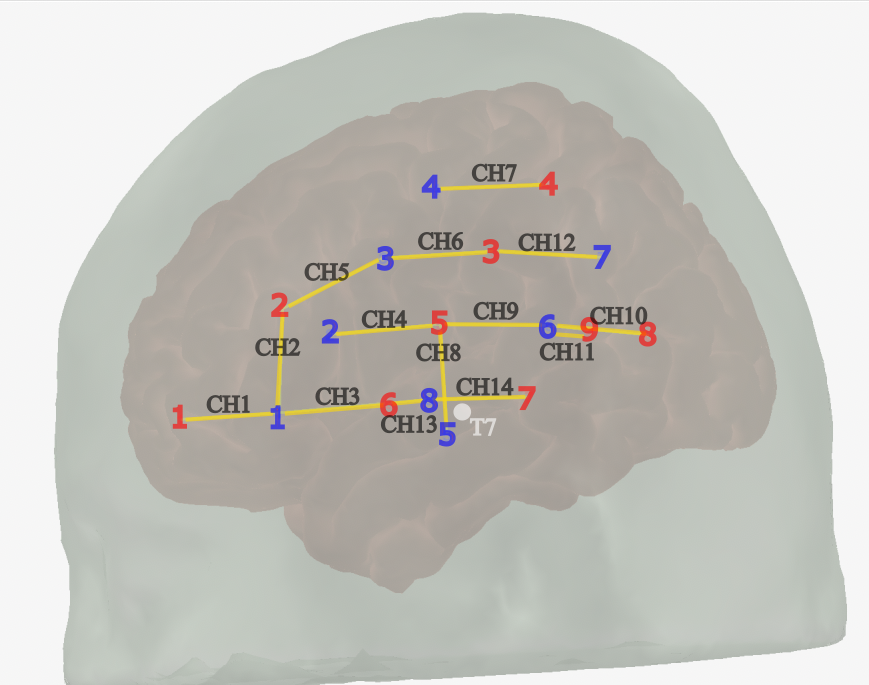
\includegraphics[scale=.45]{bilder/optode_ink.png}
  \caption{Channel Definition}
  \label{fig:somesignal}
\end{figure}

In the following figures. Channels with invalid SCI would not be taken into consideration, and hence would not be shown. Measurements in all channels were plotted in the same scale except for the two short channels marked in thicker outlines. In all our measurements, the changes in the dynamic hemoglobin response were significantly less in the short channels by more than a magnitude.

\subsection{Oxygenated Hemoglobin, HbO}
\begin{figure}[H]
  \centering
    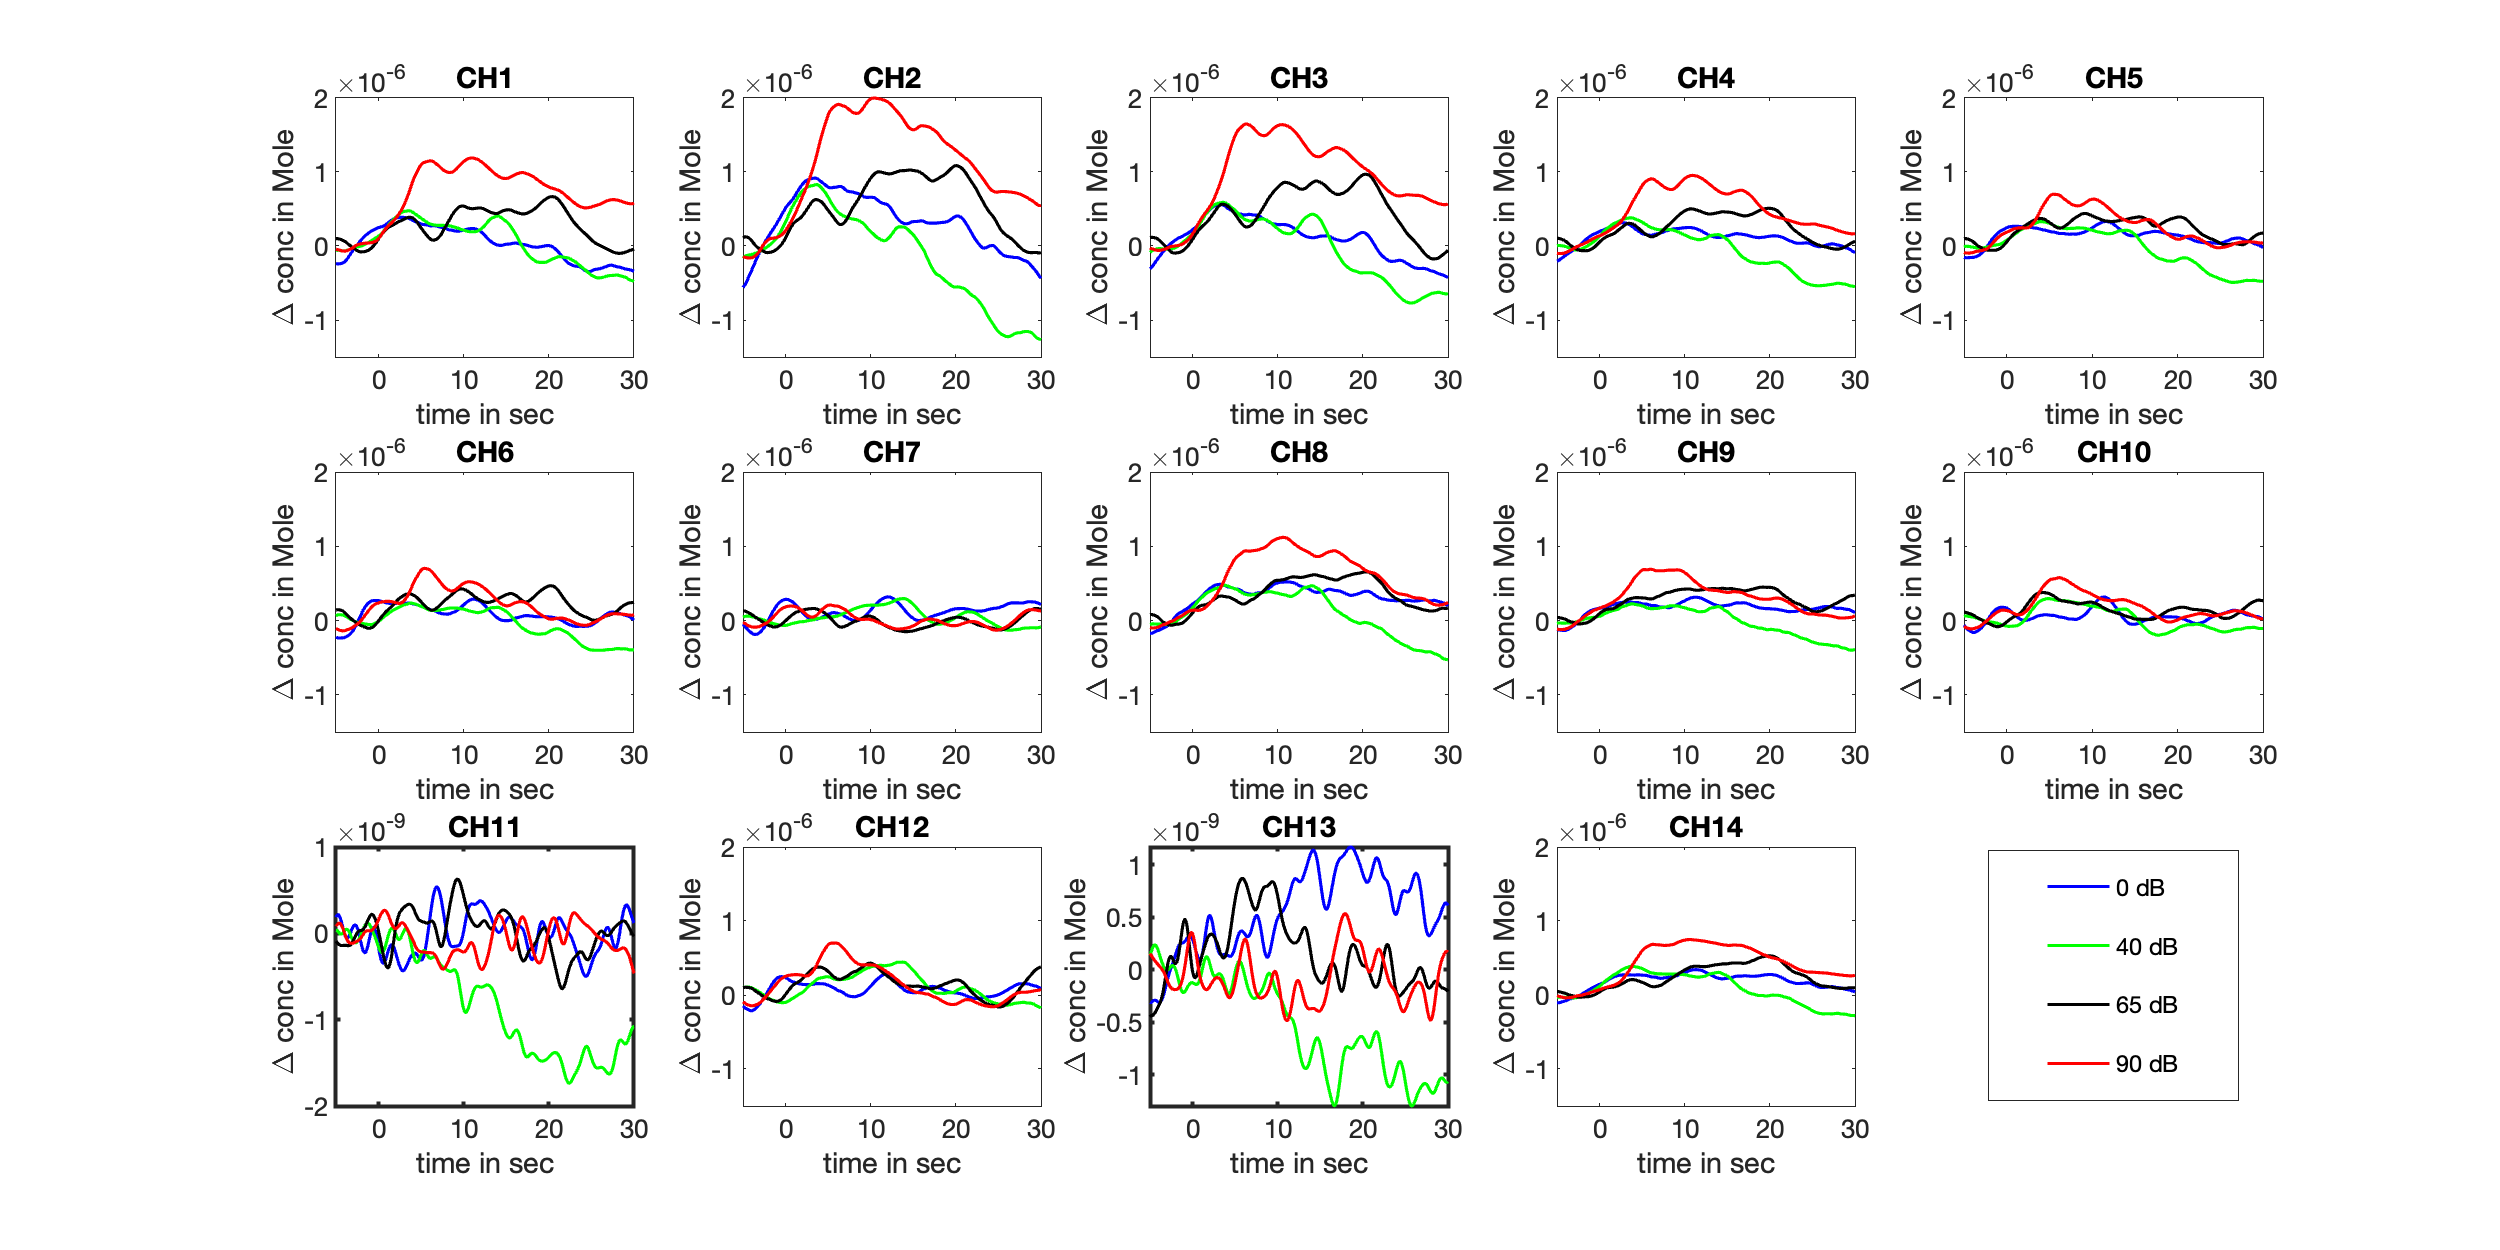
\includegraphics[scale=.4]{bilder/HbO_Mole/sub_jonas_s_HbO.png}
  \caption{Measurement from participant 3.}
  \label{fig:somesignal}
\end{figure}

\begin{figure}[H]
  \centering
    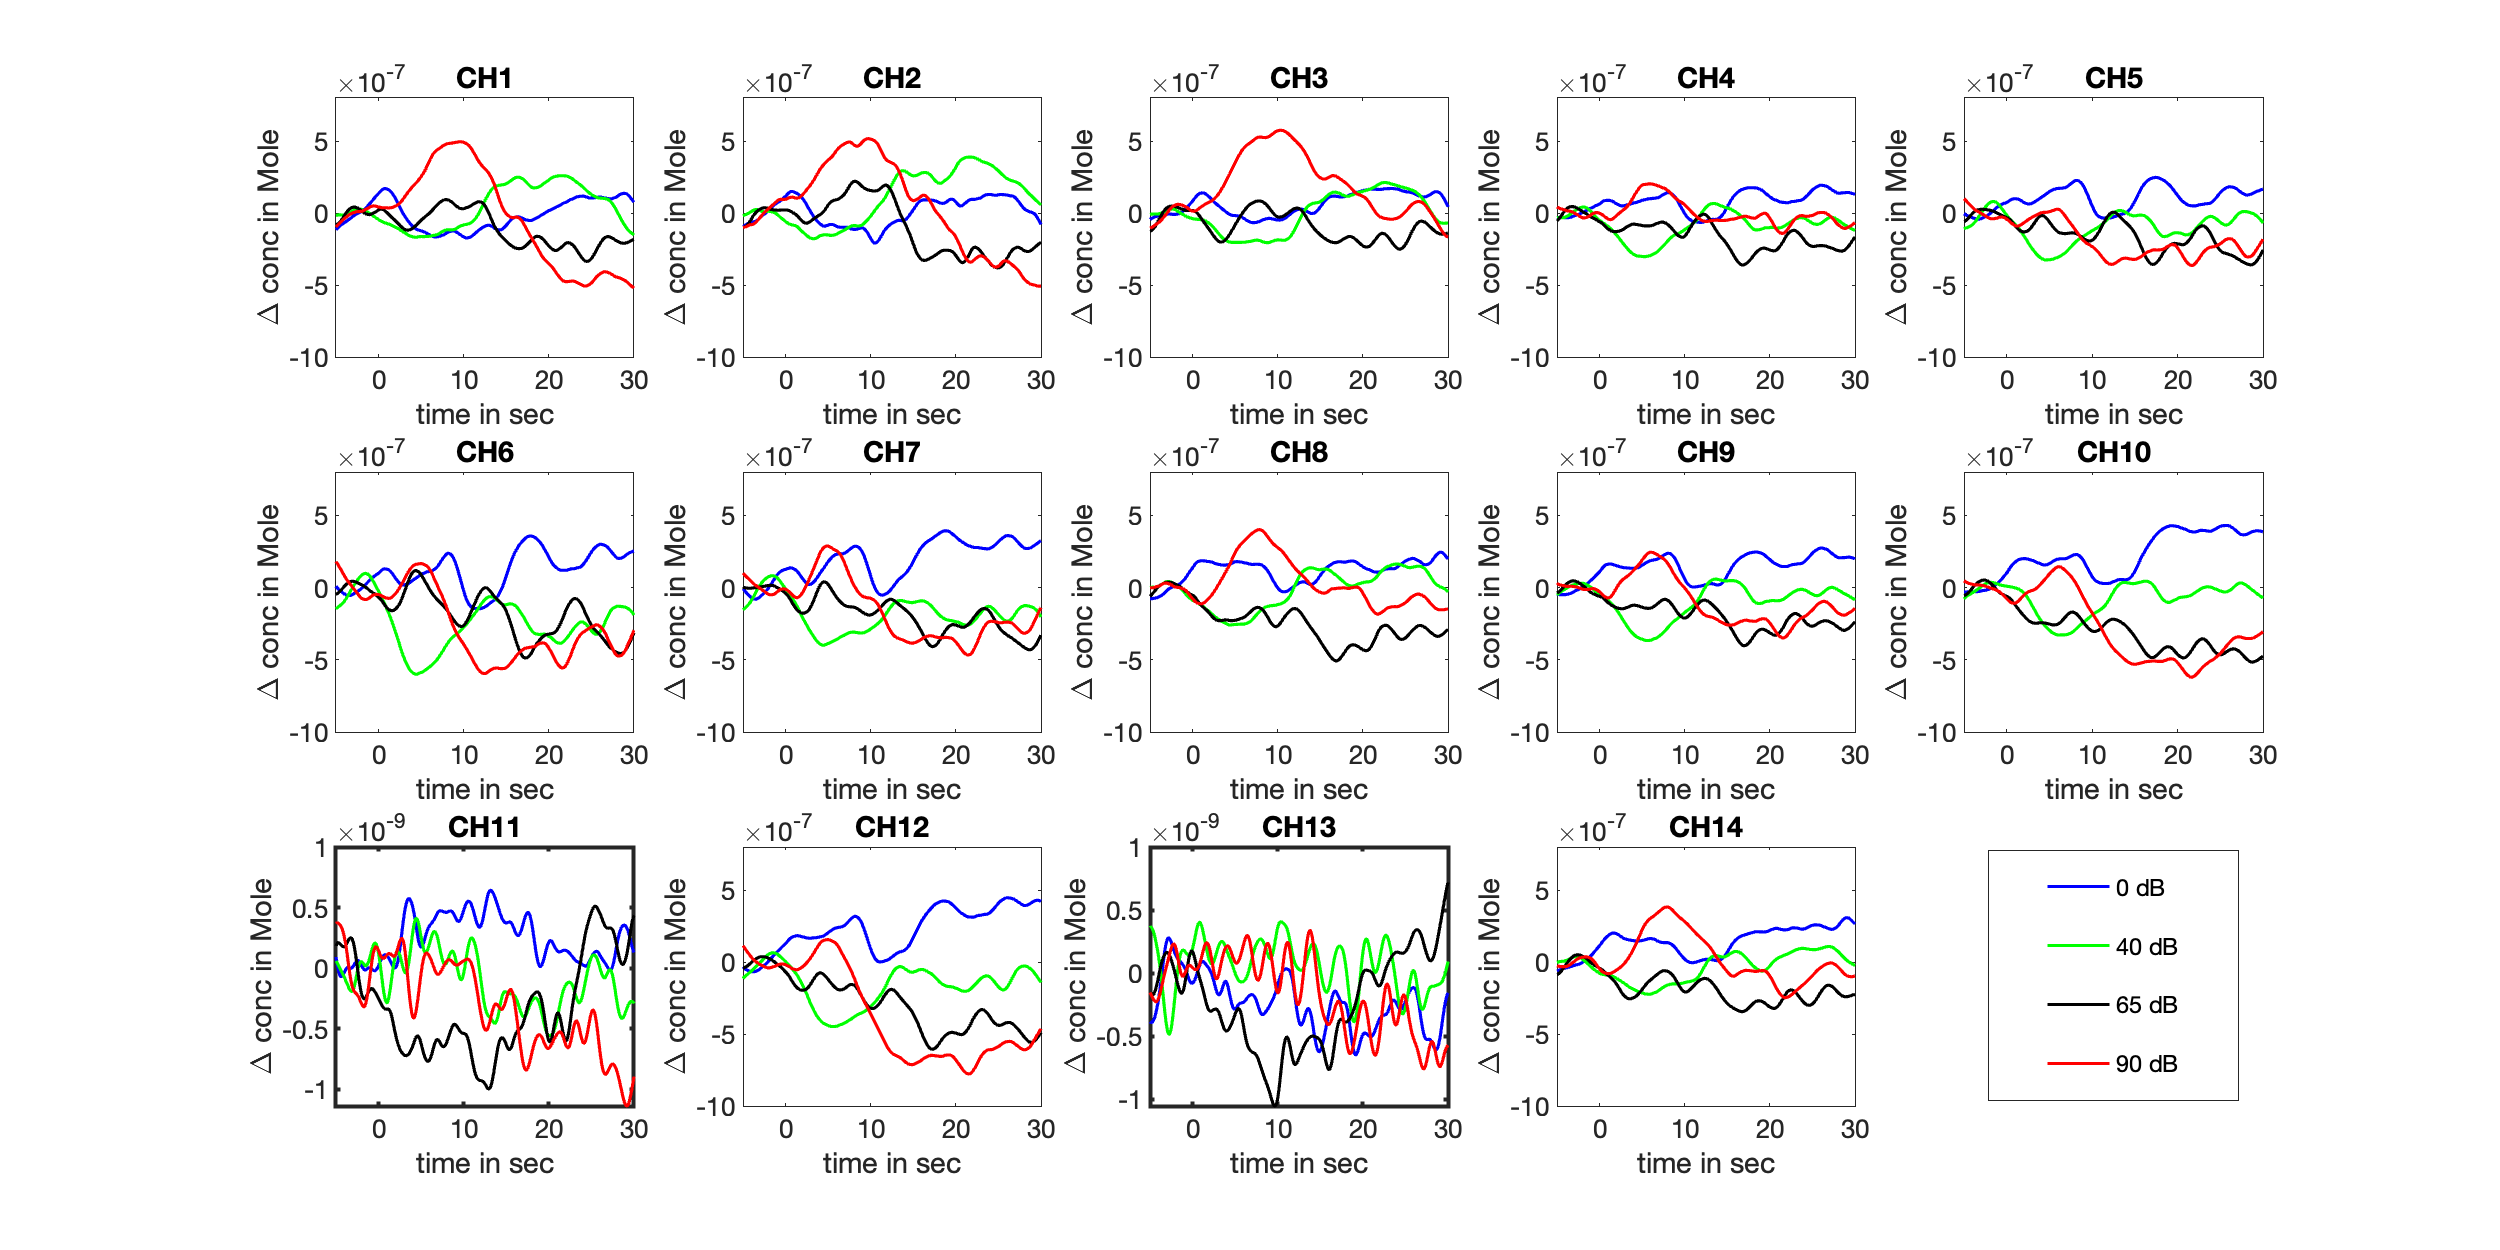
\includegraphics[scale=.4]{bilder/HbO_Mole/sub_lukas_s_HbO.png}
  \caption{Measurement from participant 5.}
  \label{fig:somesignal}
\end{figure}

\begin{figure}[H]
  \centering
    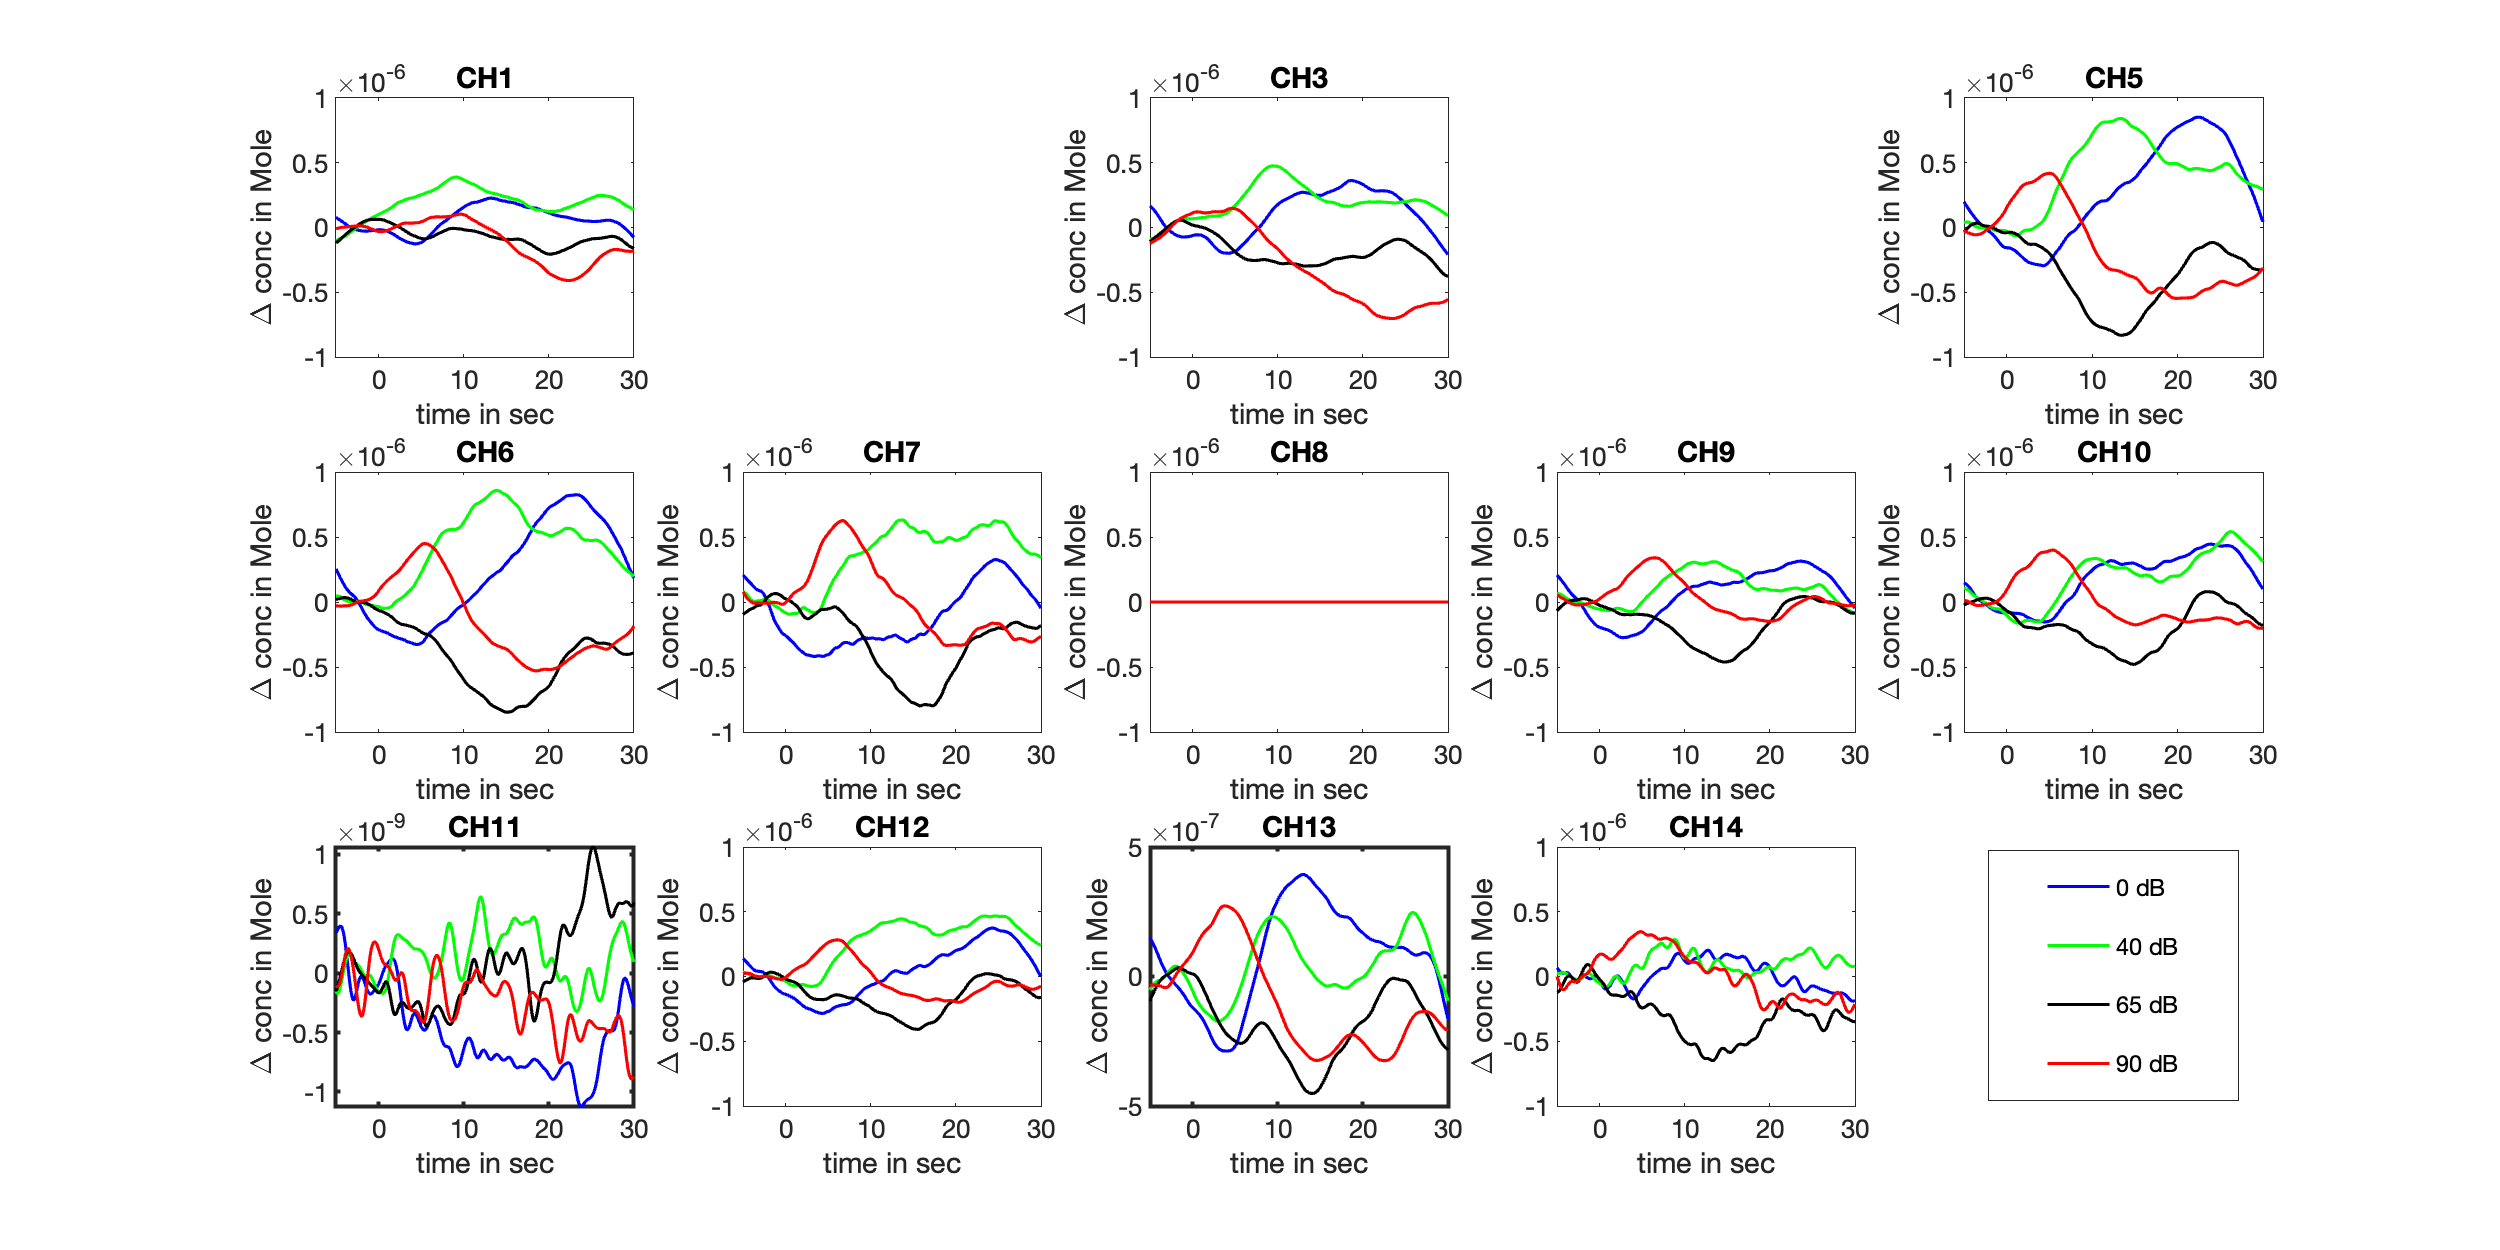
\includegraphics[scale=.4]{bilder/HbO_Mole/sub_shelia_s_HbO.png}
  \caption{Measurement from participant 6.}
  \label{fig:somesignal}
\end{figure}

\begin{figure}[H]
  \centering
    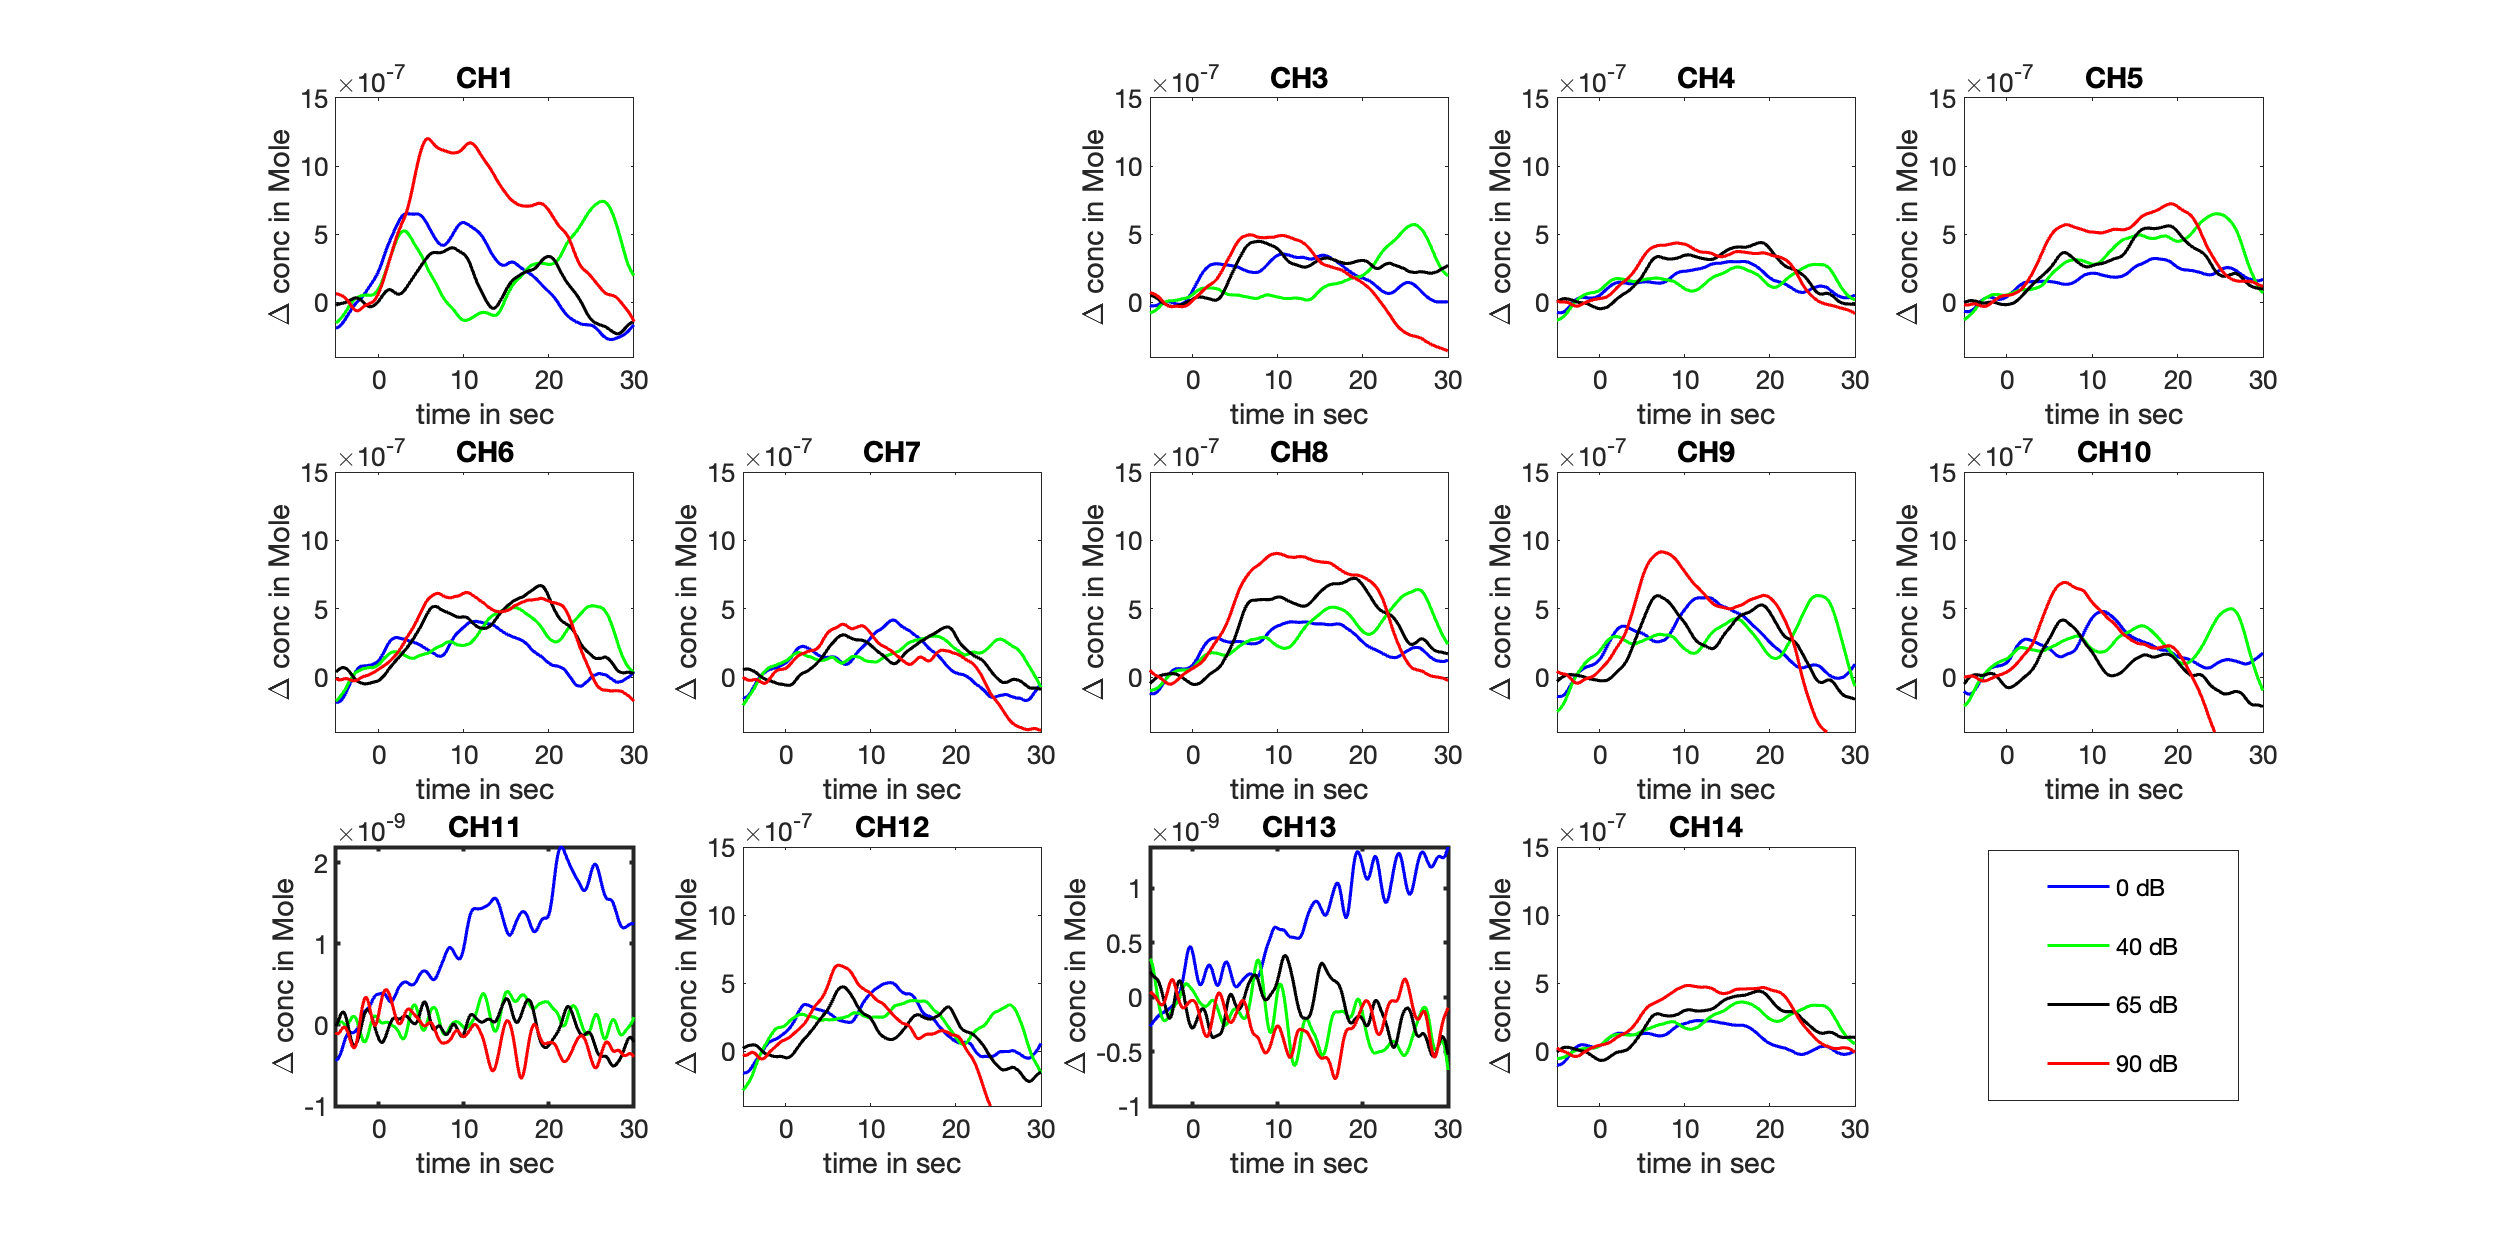
\includegraphics[scale=.4]{bilder/HbO_Mole/sub_liao_s_HbO.png}
  \caption{Measurement from participant 7.}
  \label{fig:somesignal}
\end{figure}


\begin{figure}[H]
  \centering
    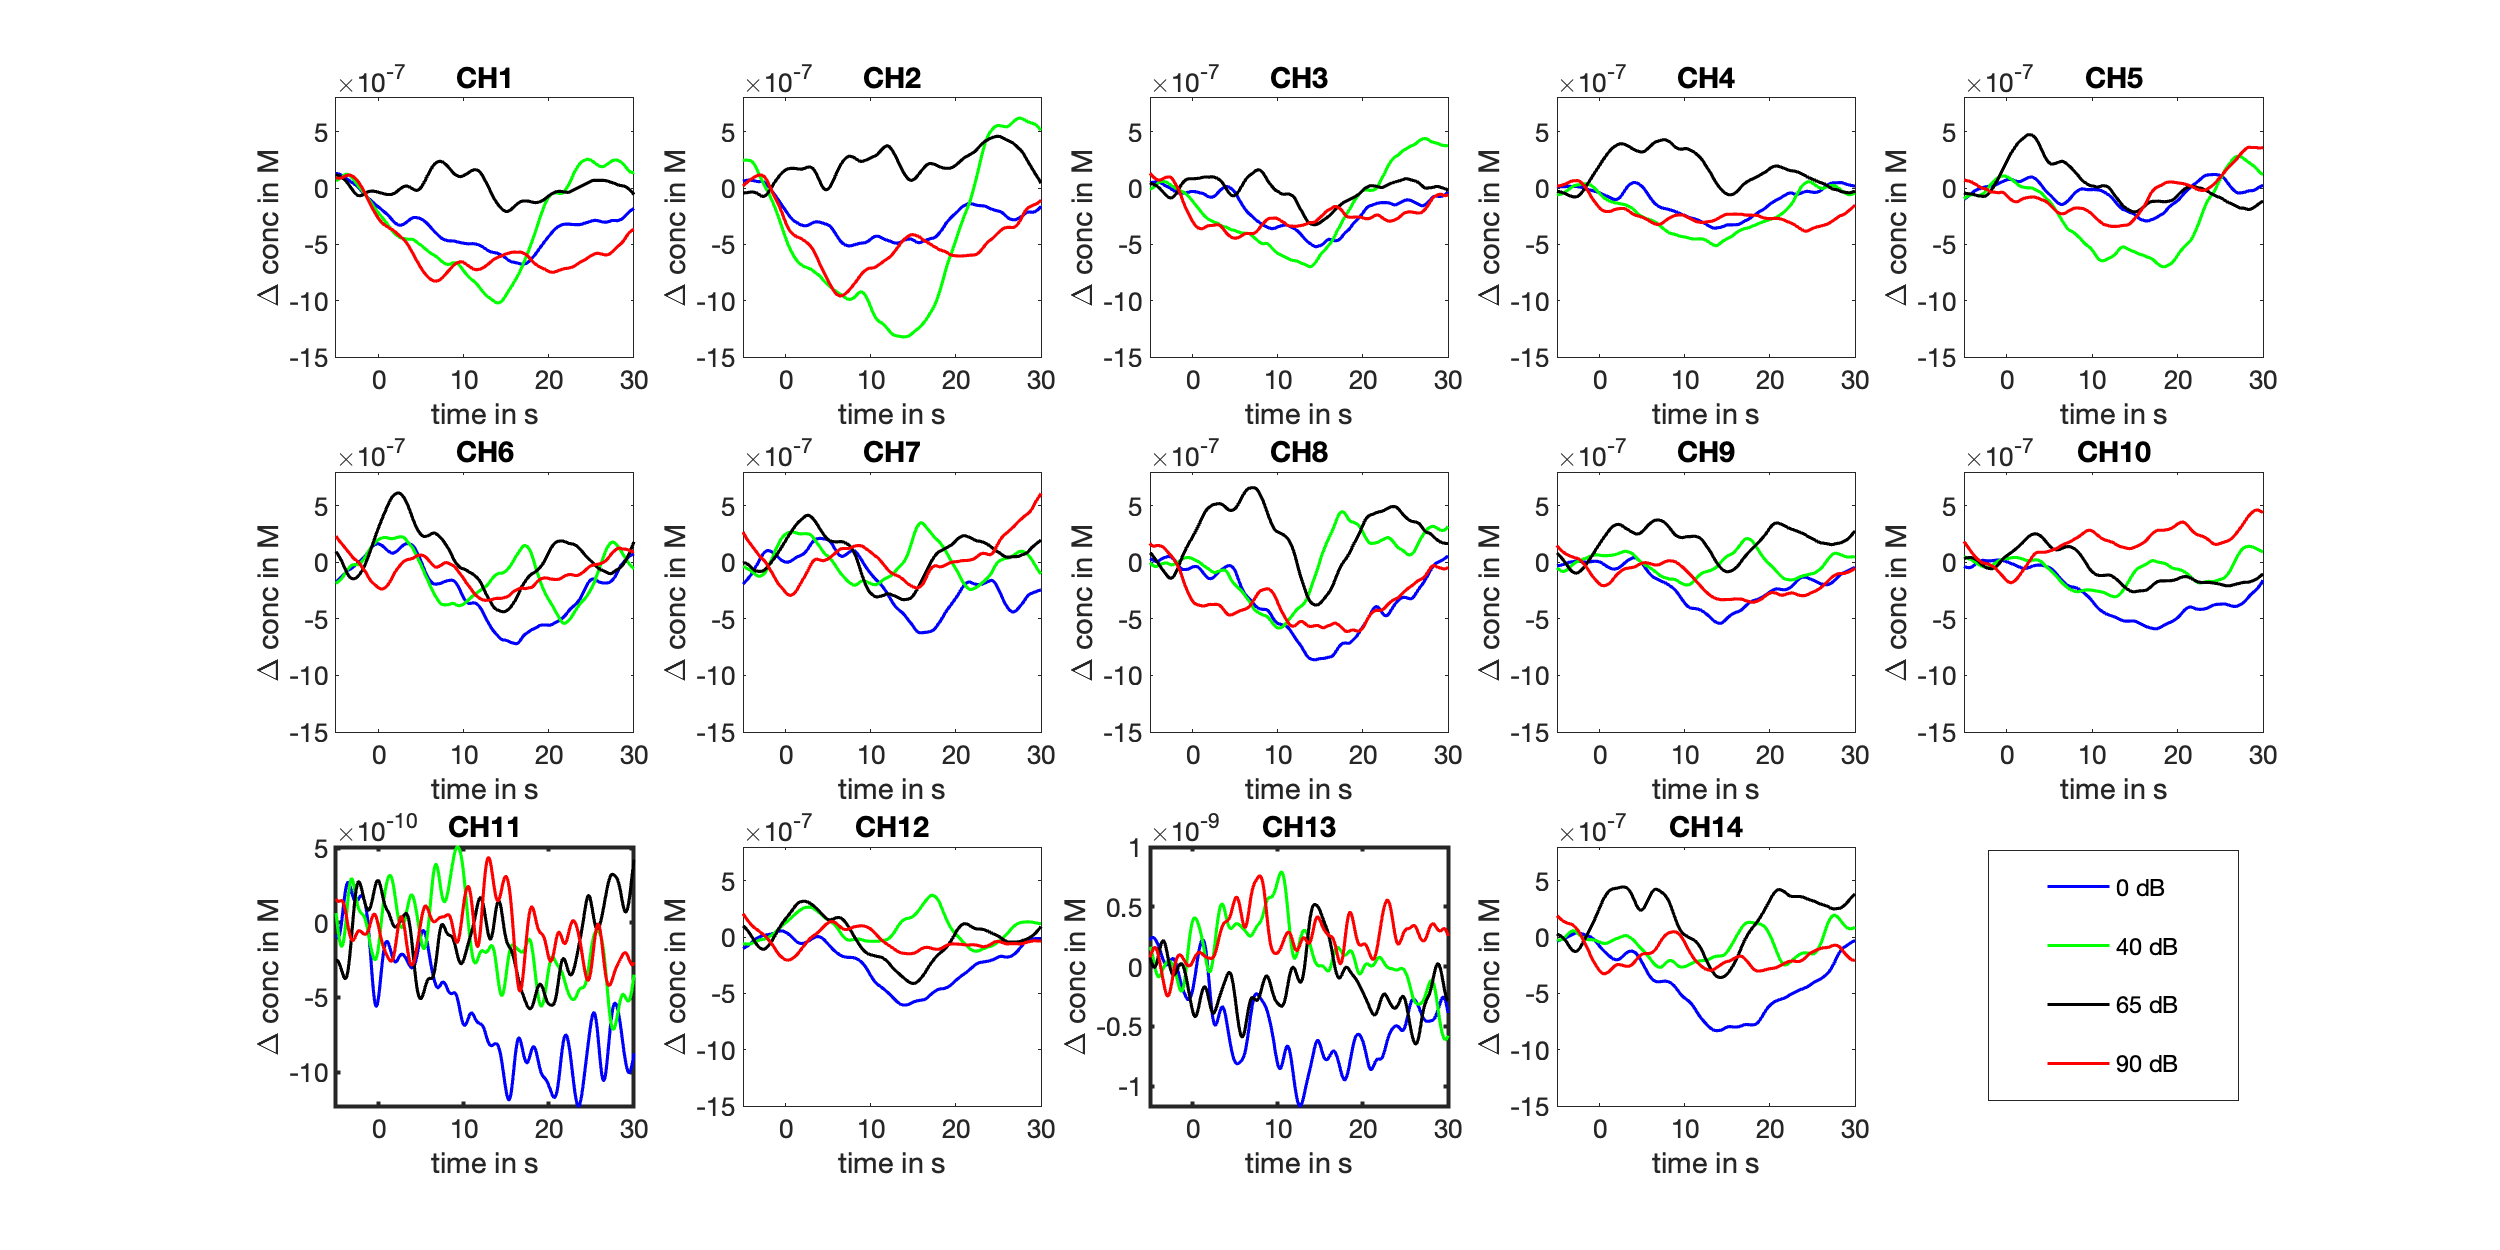
\includegraphics[scale=.4]{bilder/HbO_Mole/sub_luca2_s_HbO.png}
  \caption{Measurement from participant 8. Silent comparison}
  \label{fig:somesignal}
\end{figure}



\newpage

\subsection{Deoxygenated Hemoglobin, HbR}

\begin{figure}[H]
  \centering
    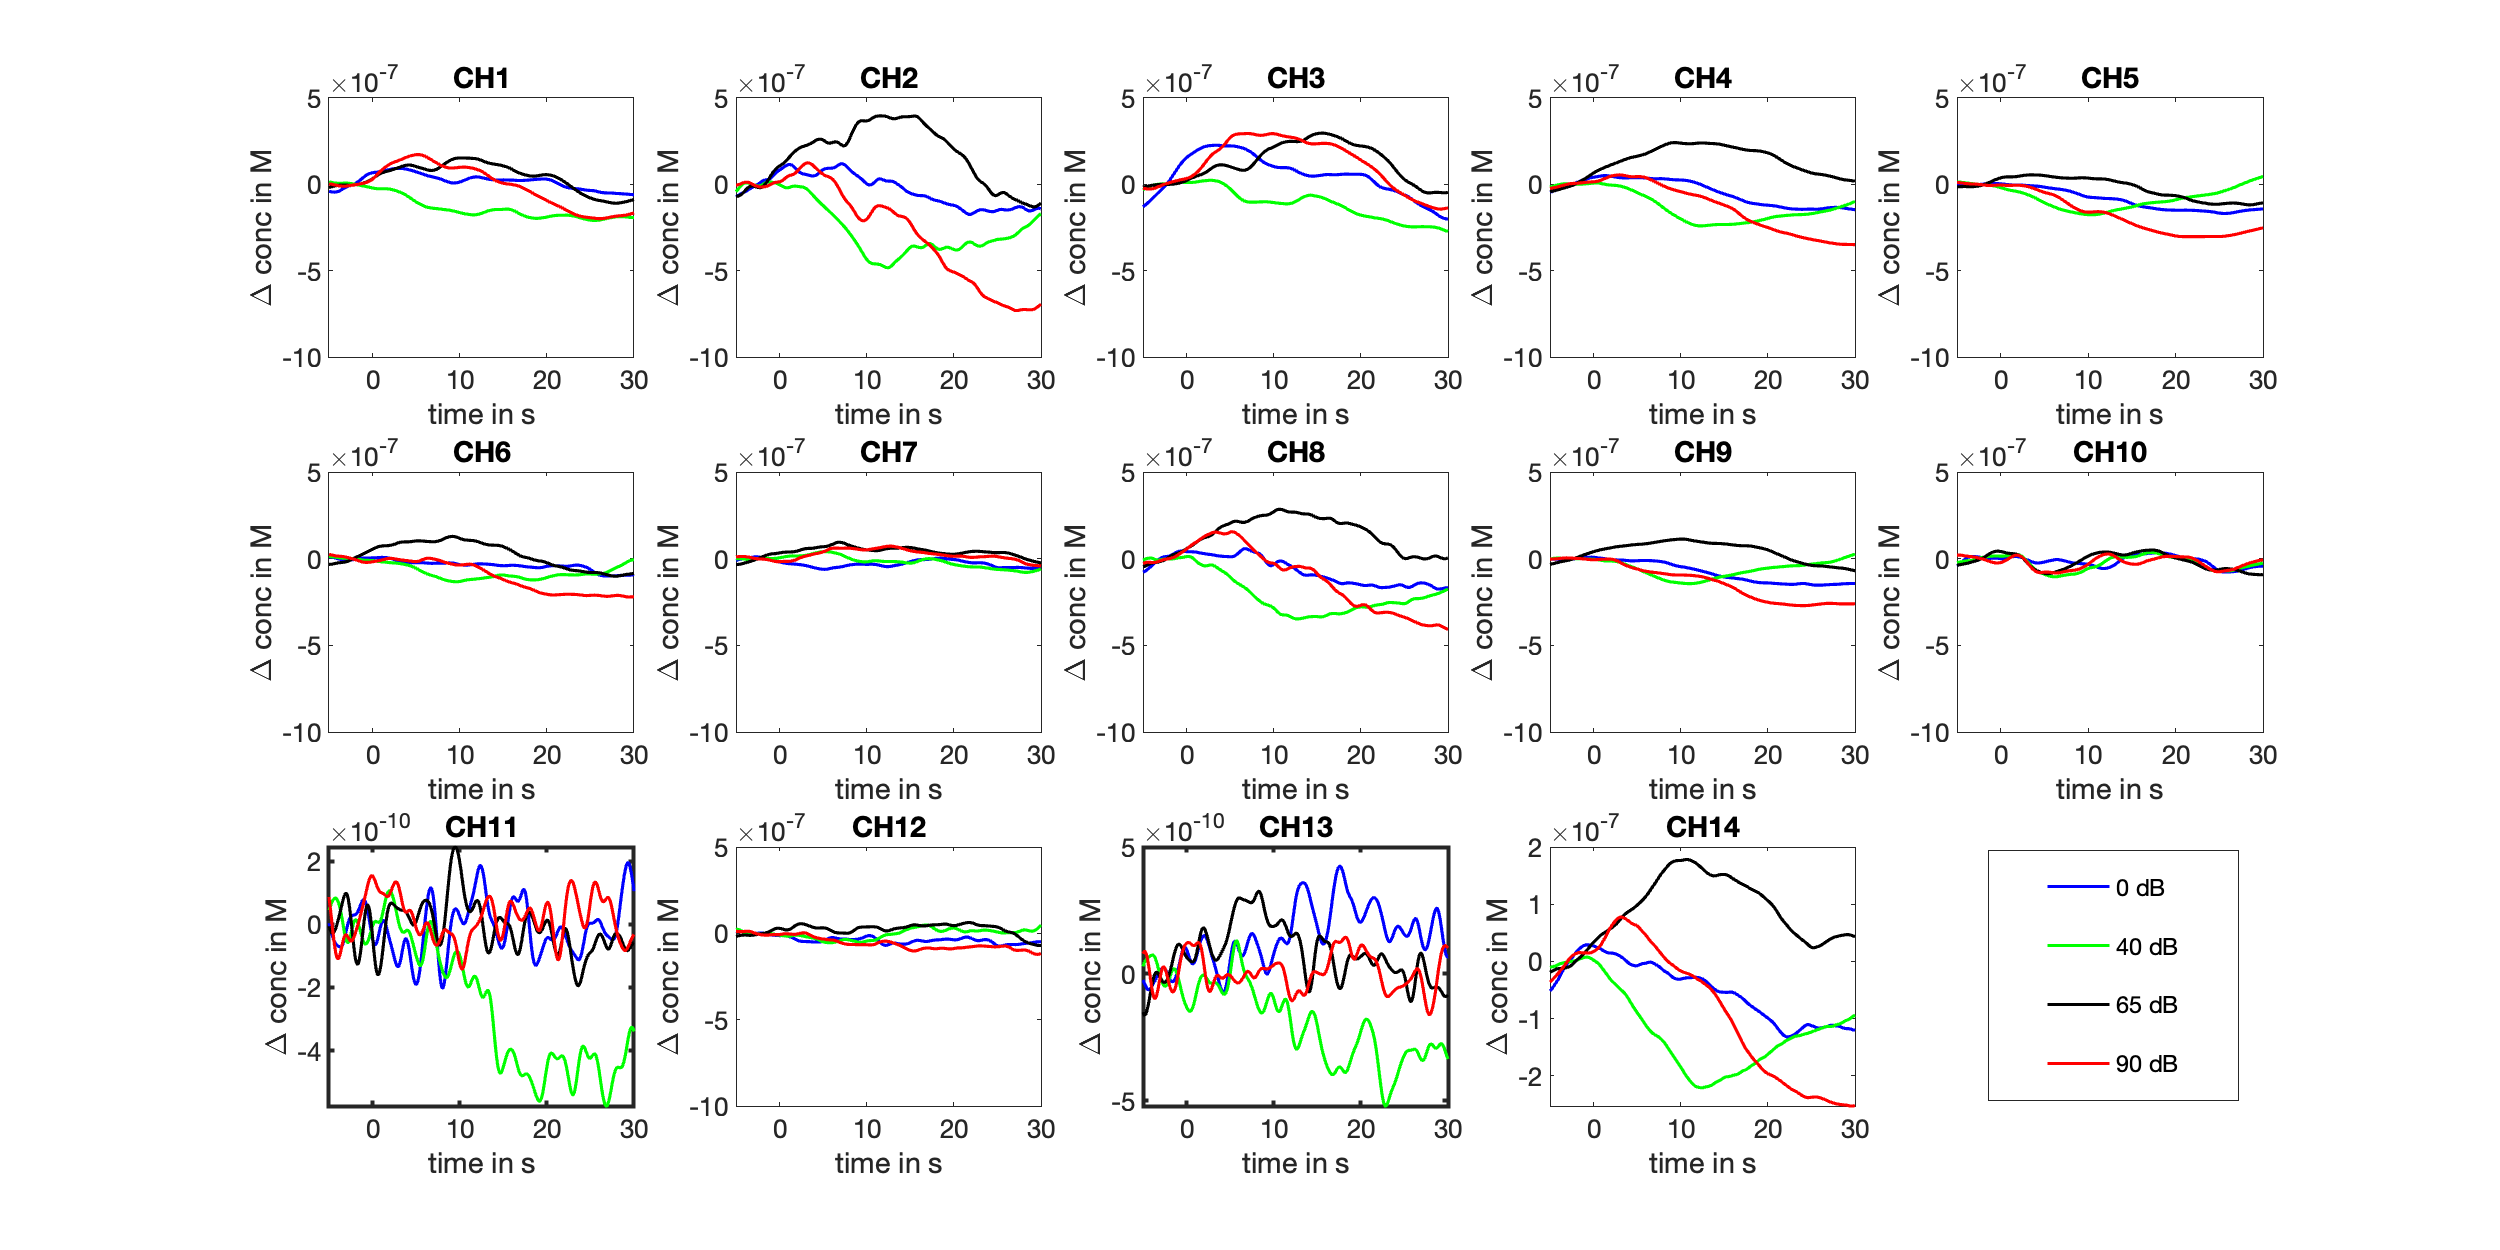
\includegraphics[scale=.4]{bilder/HbR_Mole/sub_jonas_s_HbR.png}
  \caption{Measurement from participant 3.}
  \label{fig:somesignal}
\end{figure}

\begin{figure}[H]
  \centering
    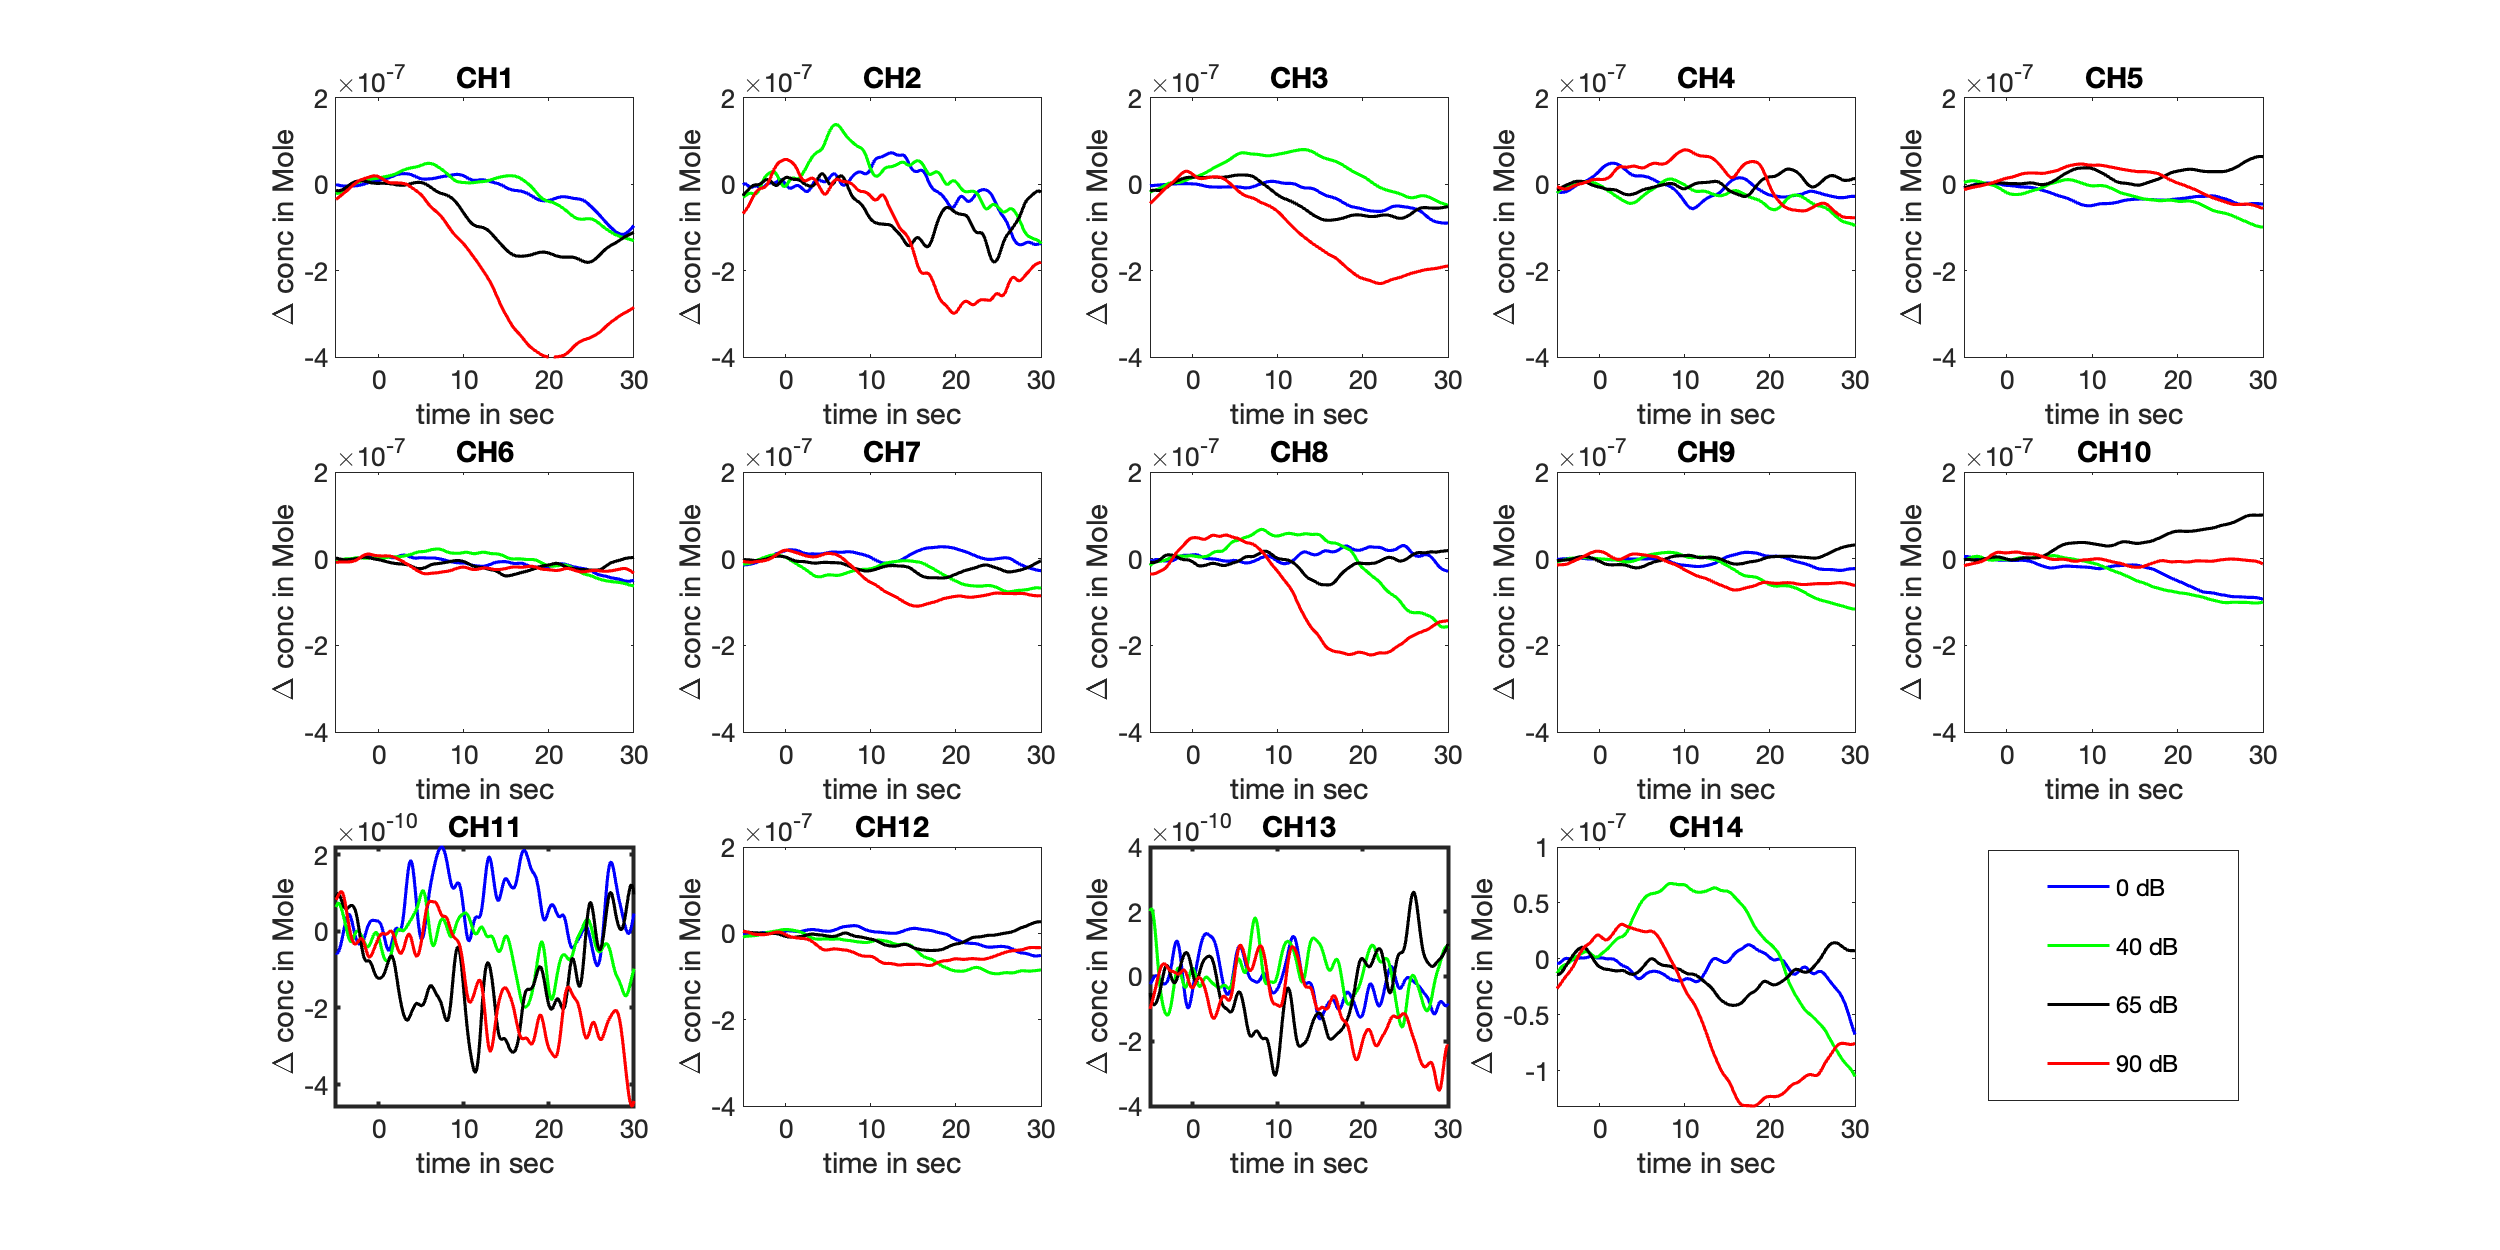
\includegraphics[scale=.4]{bilder/HbR_Mole/sub_lukas_s_HbR.png}
  \caption{Measurement from participant 5.}
  \label{fig:somesignal}
\end{figure}

\begin{figure}[H]
  \centering
    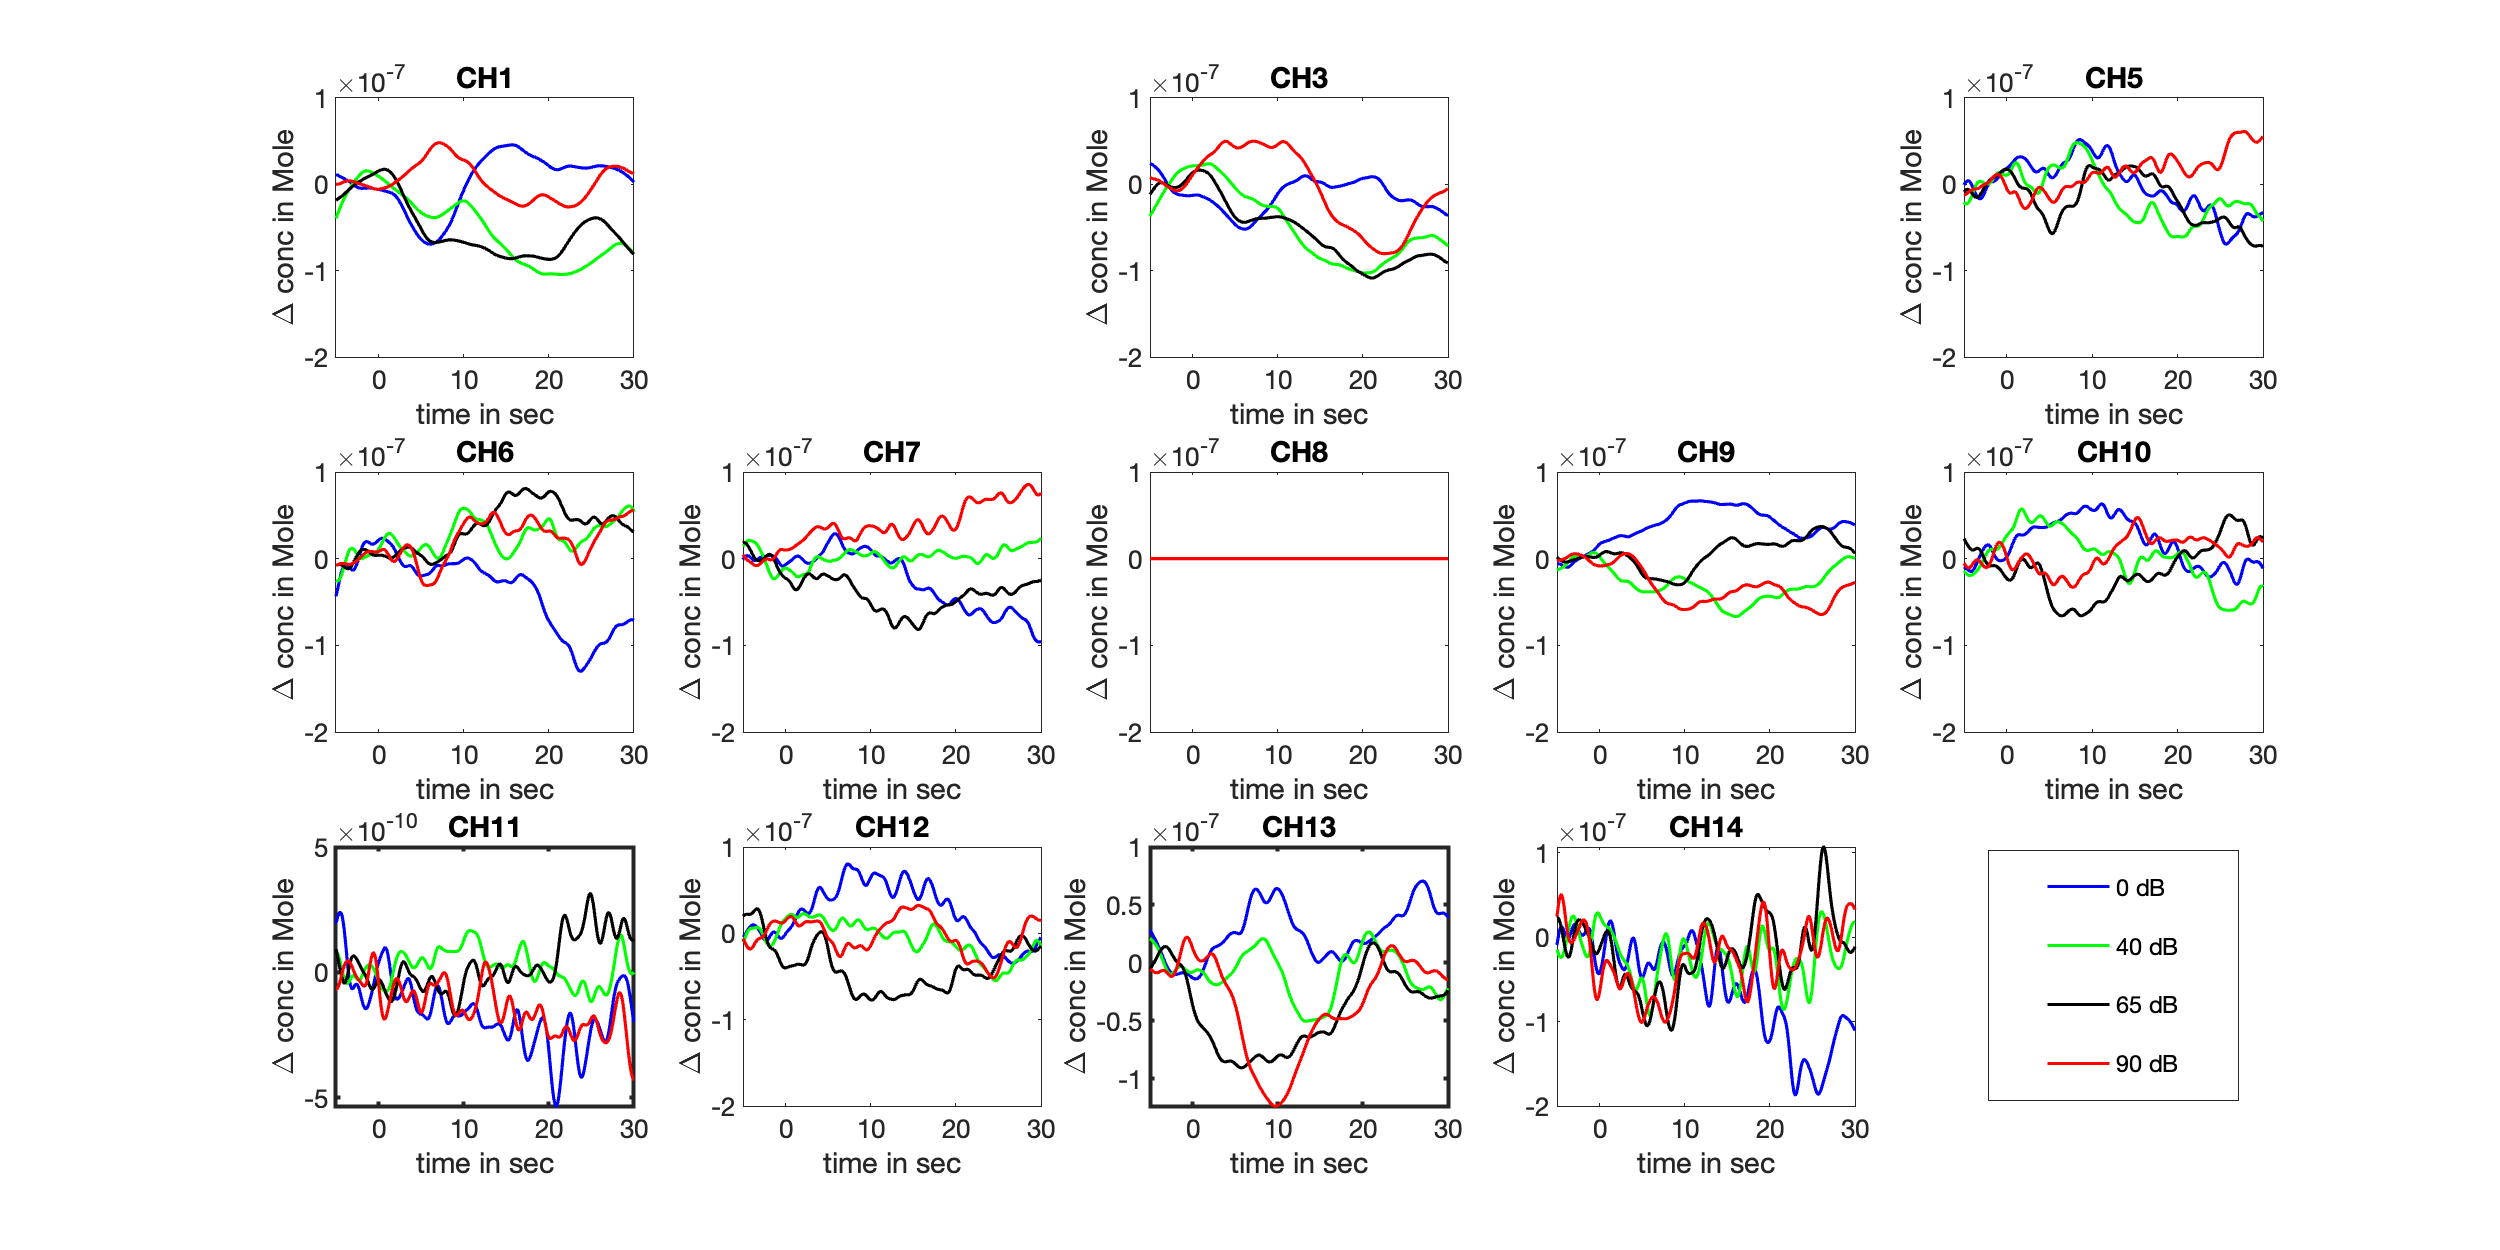
\includegraphics[scale=.4]{bilder/HbR_Mole/sub_shelia_s_HbR.png}
  \caption{Measurement from participant 6.}
  \label{fig:somesignal}
\end{figure}

\begin{figure}[H]
  \centering
    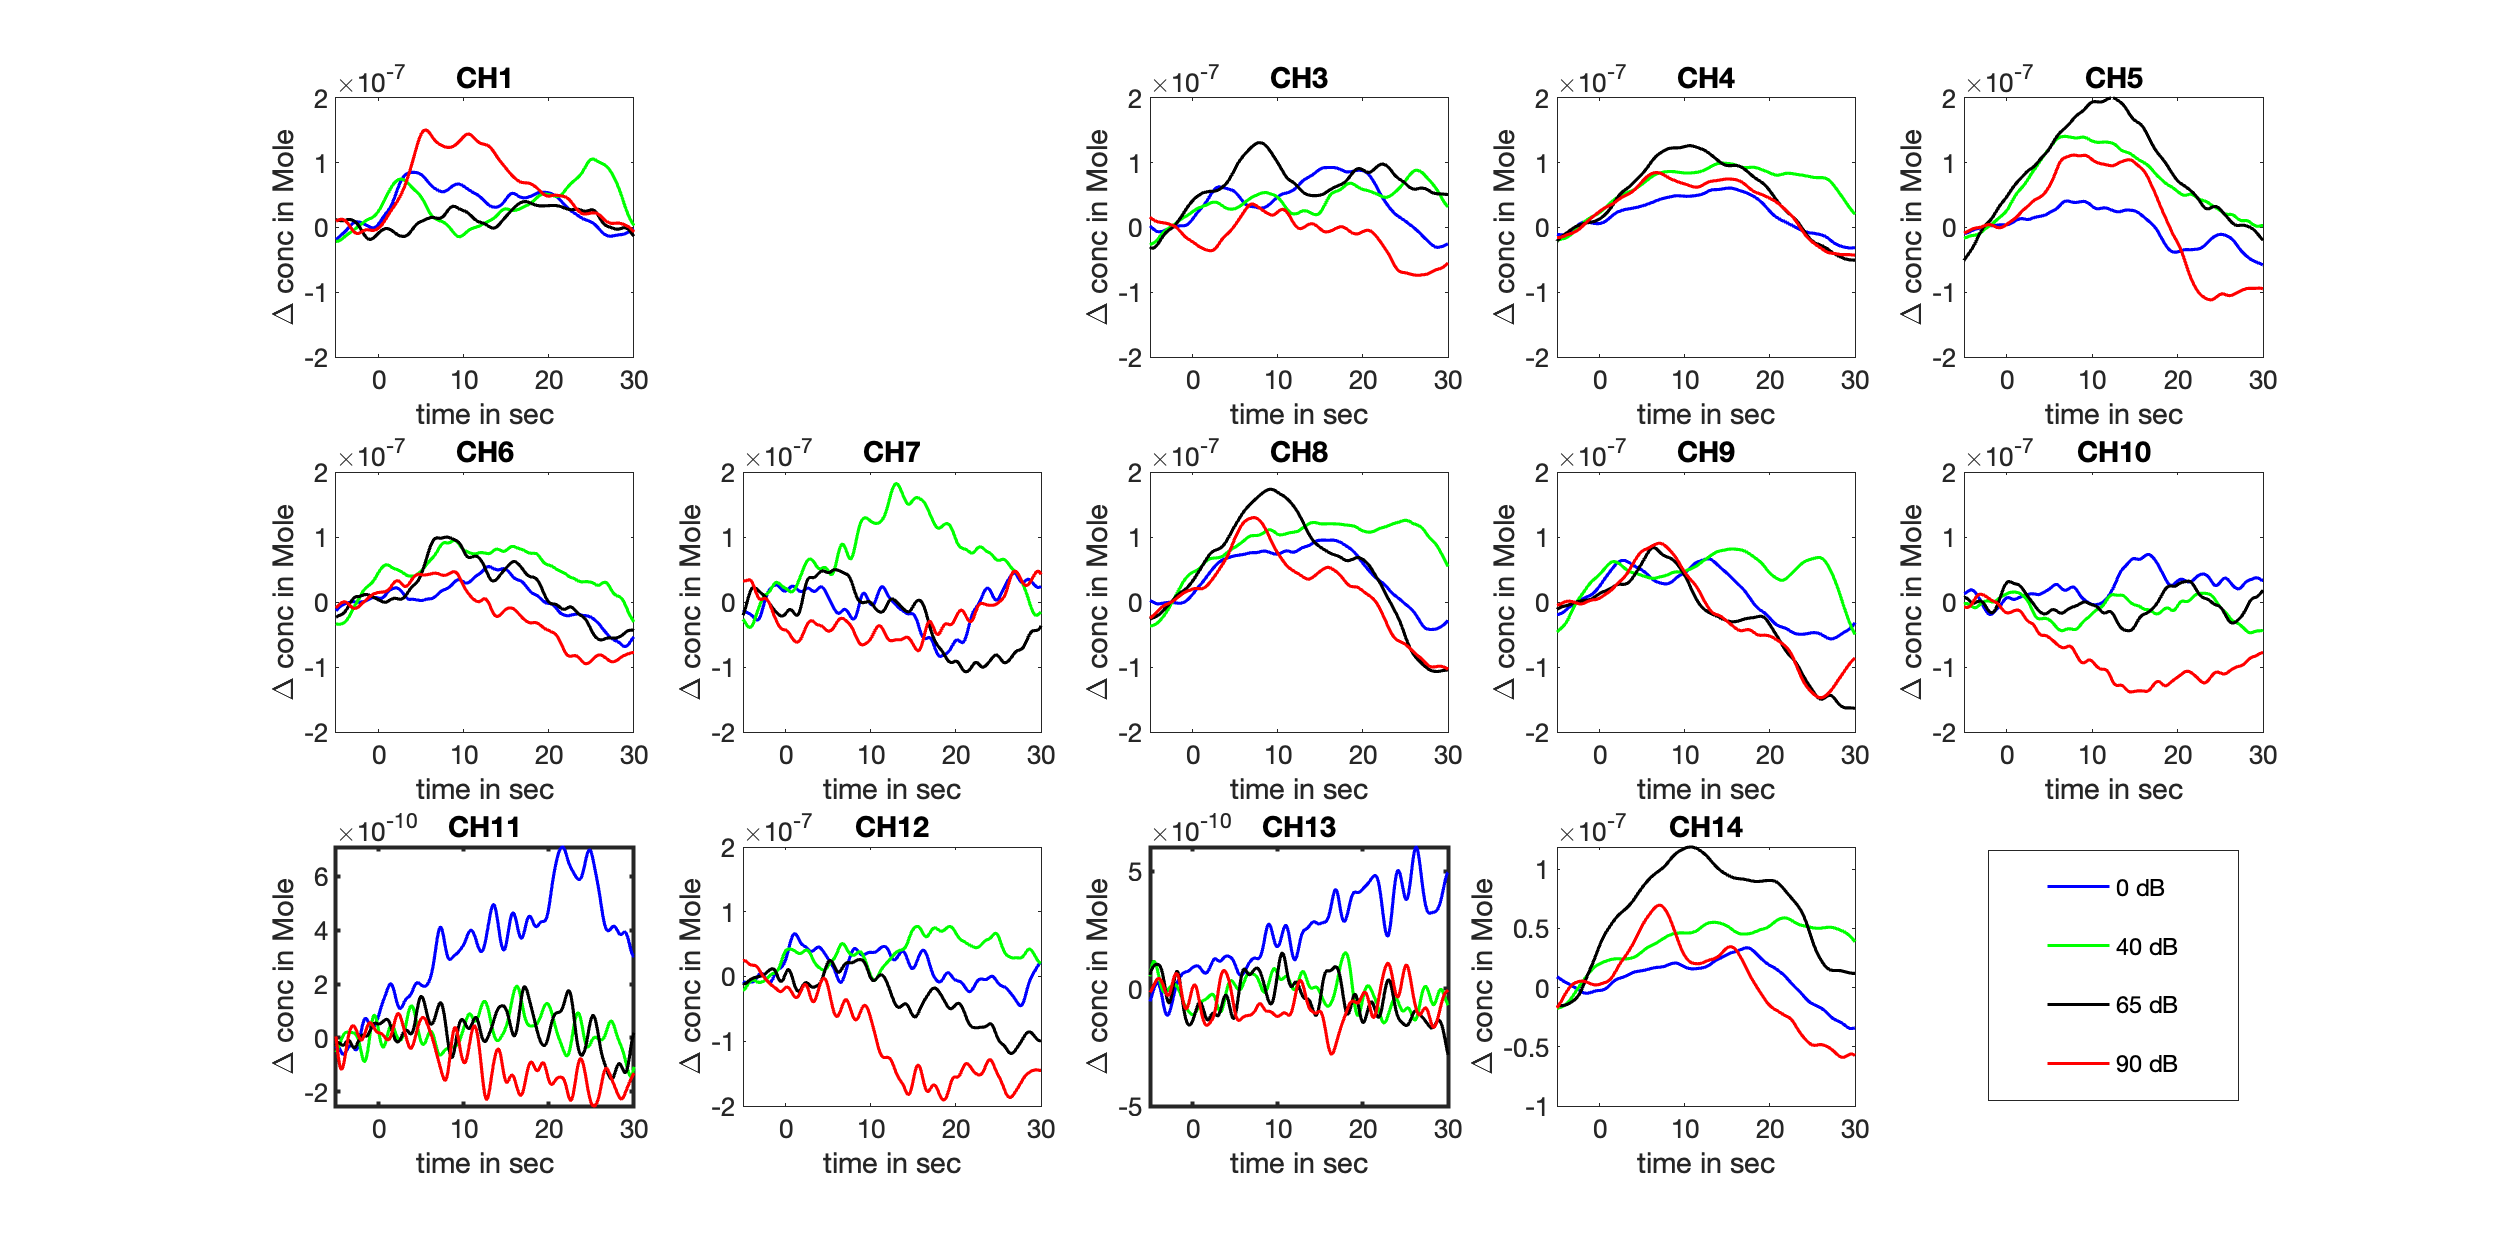
\includegraphics[scale=.4]{bilder/HbR_Mole/sub_liao_s_HbR.png}
  \caption{Measurement from participant 7.}
  \label{fig:somesignal}
\end{figure}


\begin{figure}[H]
  \centering
    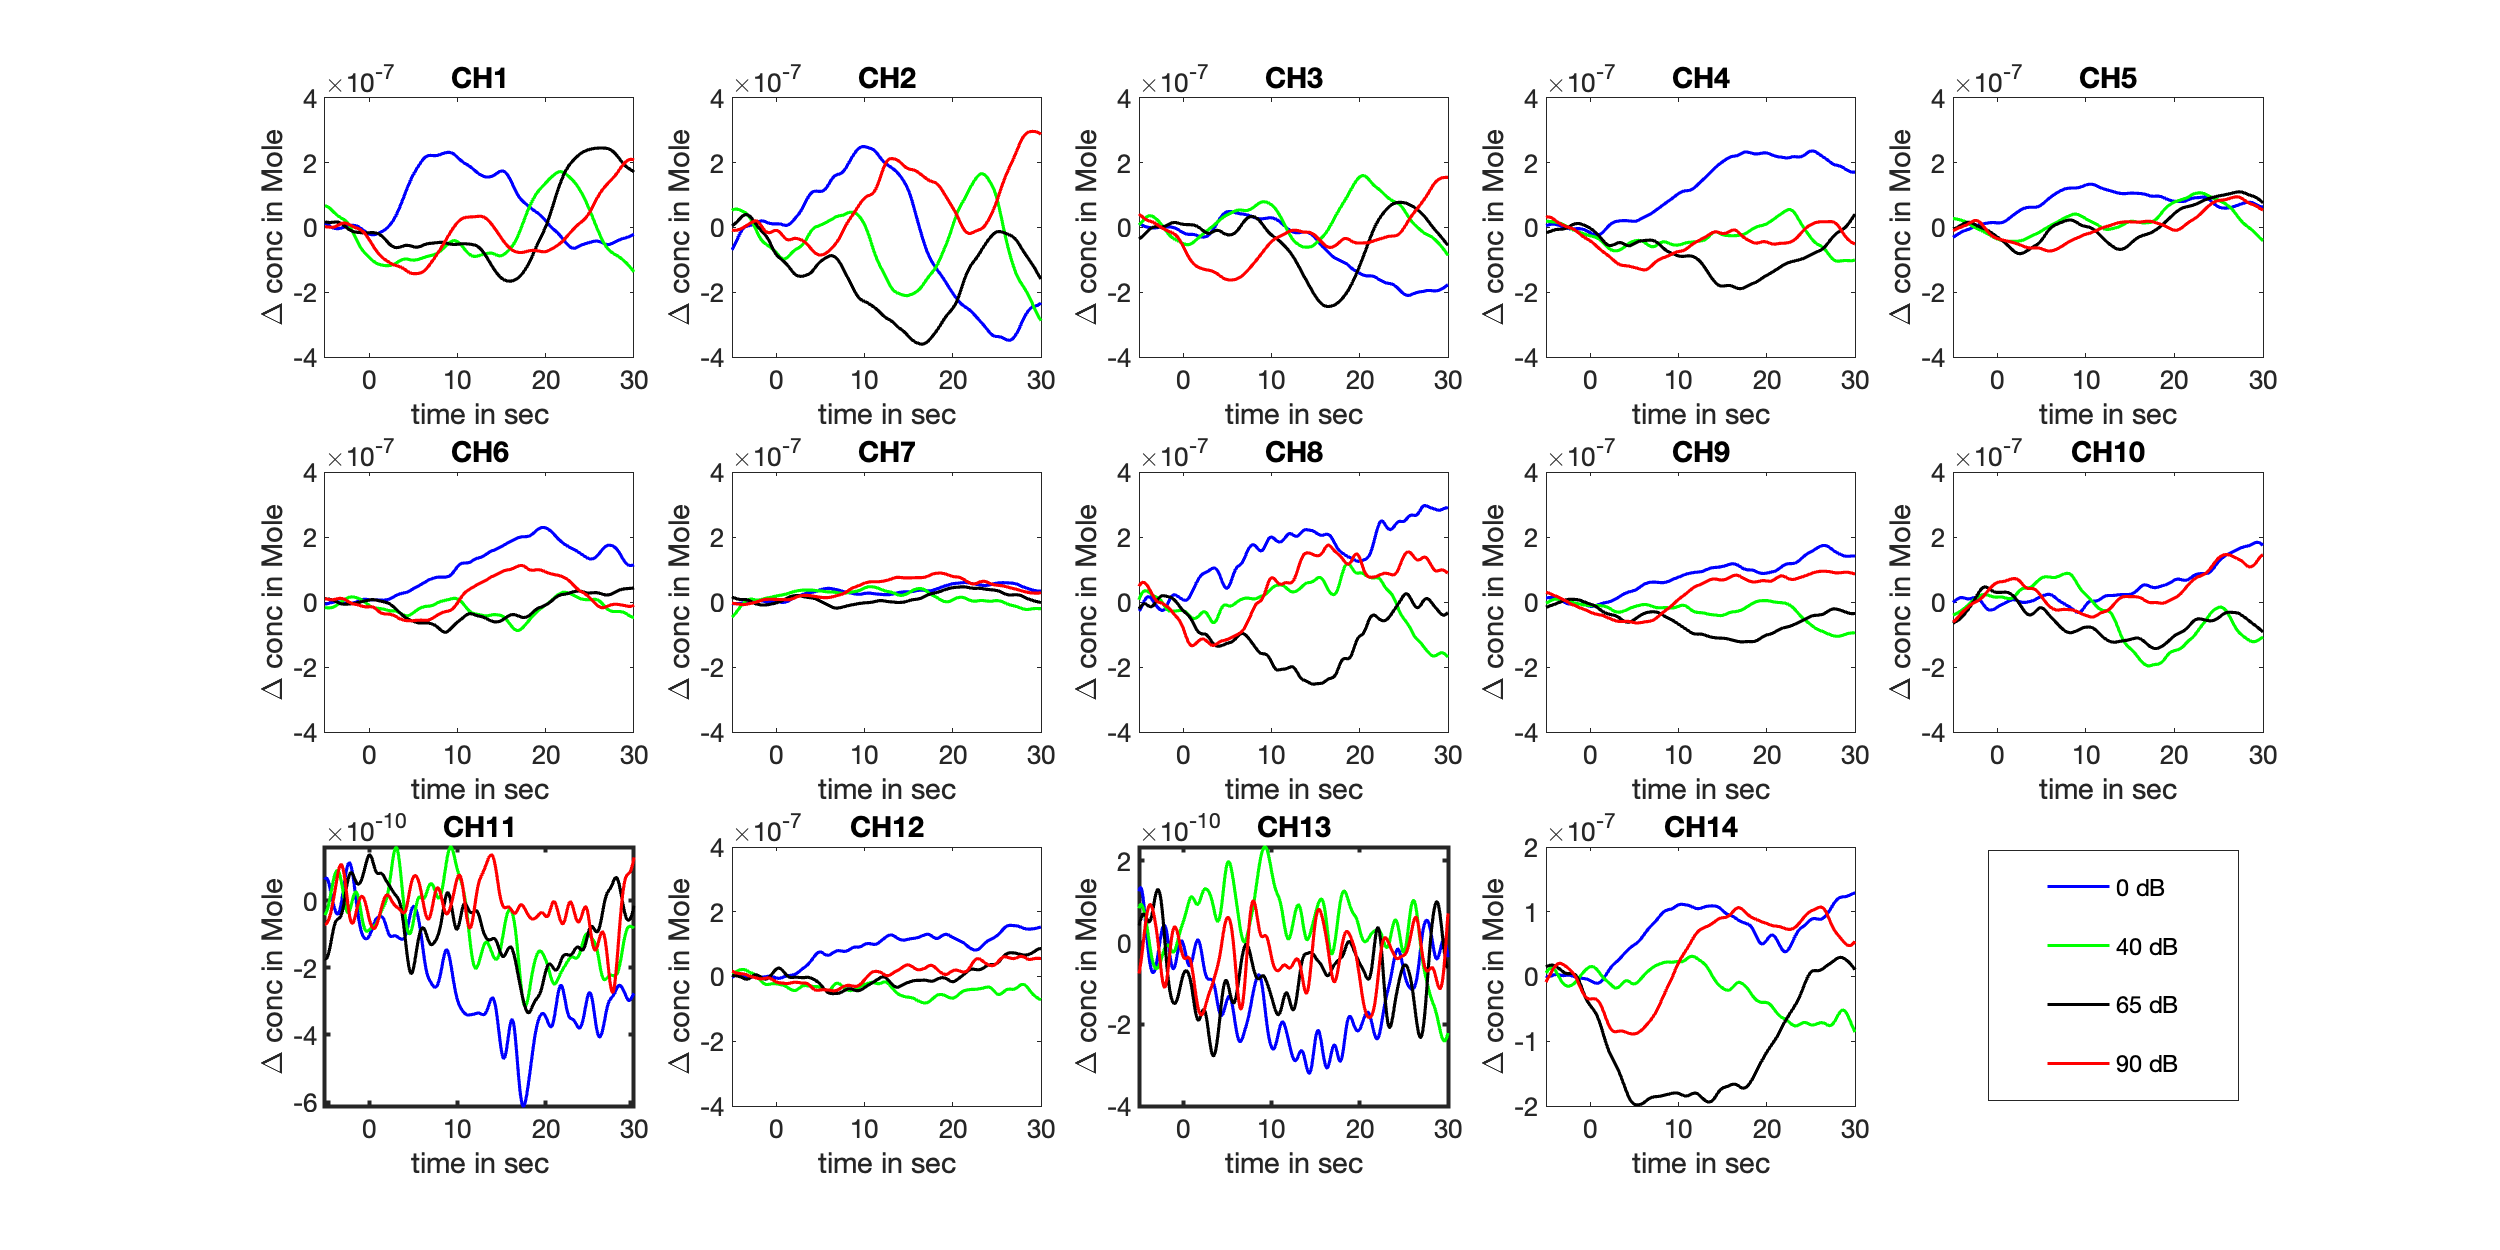
\includegraphics[scale=.4]{bilder/HbR_Mole/sub_luca2_s_HbR.png}
  \caption{Measurement from participant 8. Silent comparison}
\end{figure}





\section {Region of Interest}
In the following, regions of interest (ROI) are defined as the following figures. The auditory cortex is in particular of our interest. Hence, channel 4, channel 8, and channel 9 together formed one region (ROI 2). The rest of the channels formed ROI 1. It is of our interest to compare how the response of the auditory cortex differ from the rest of the left brain hemisphere.

\begin{figure}[H]
  \centering
    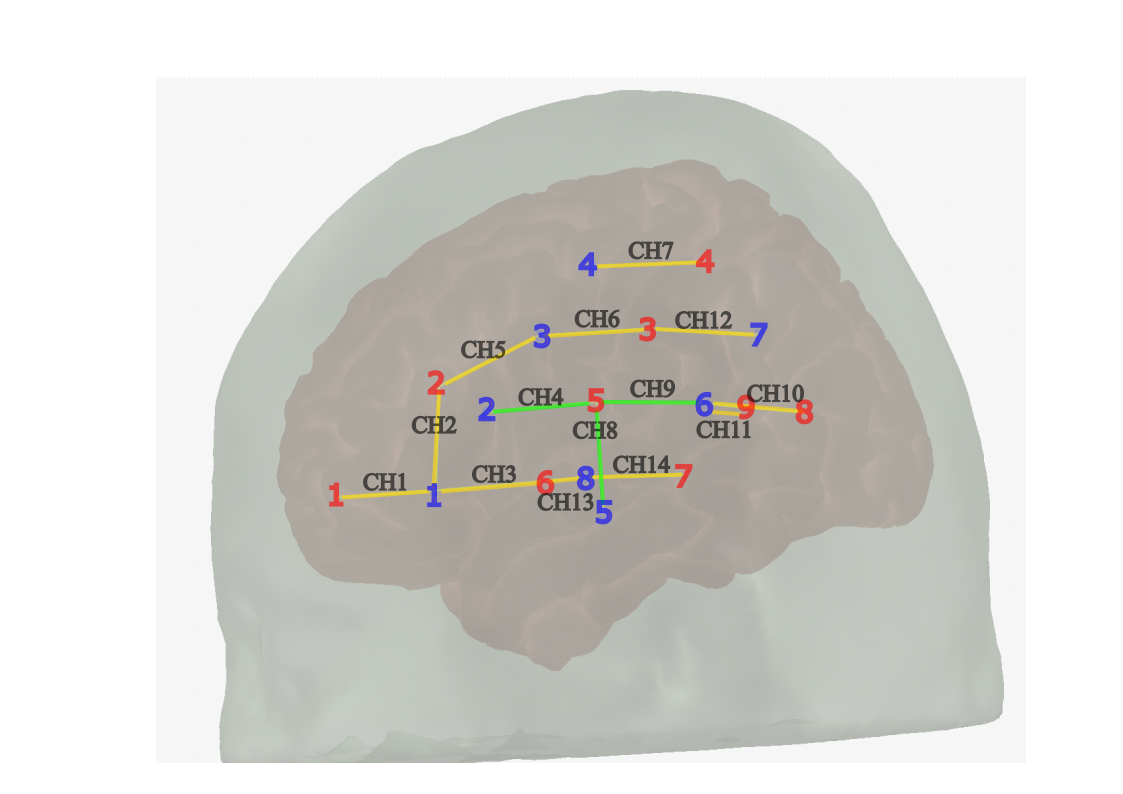
\includegraphics[scale=.45]{bilder/optode_roi_ink.png}
  \caption{ROI Definition}
\end{figure}



The following plots shows the averaged \textbf {HbO} response of all the valid channels in the defined region.
\begin{figure}[H]
  \centering
    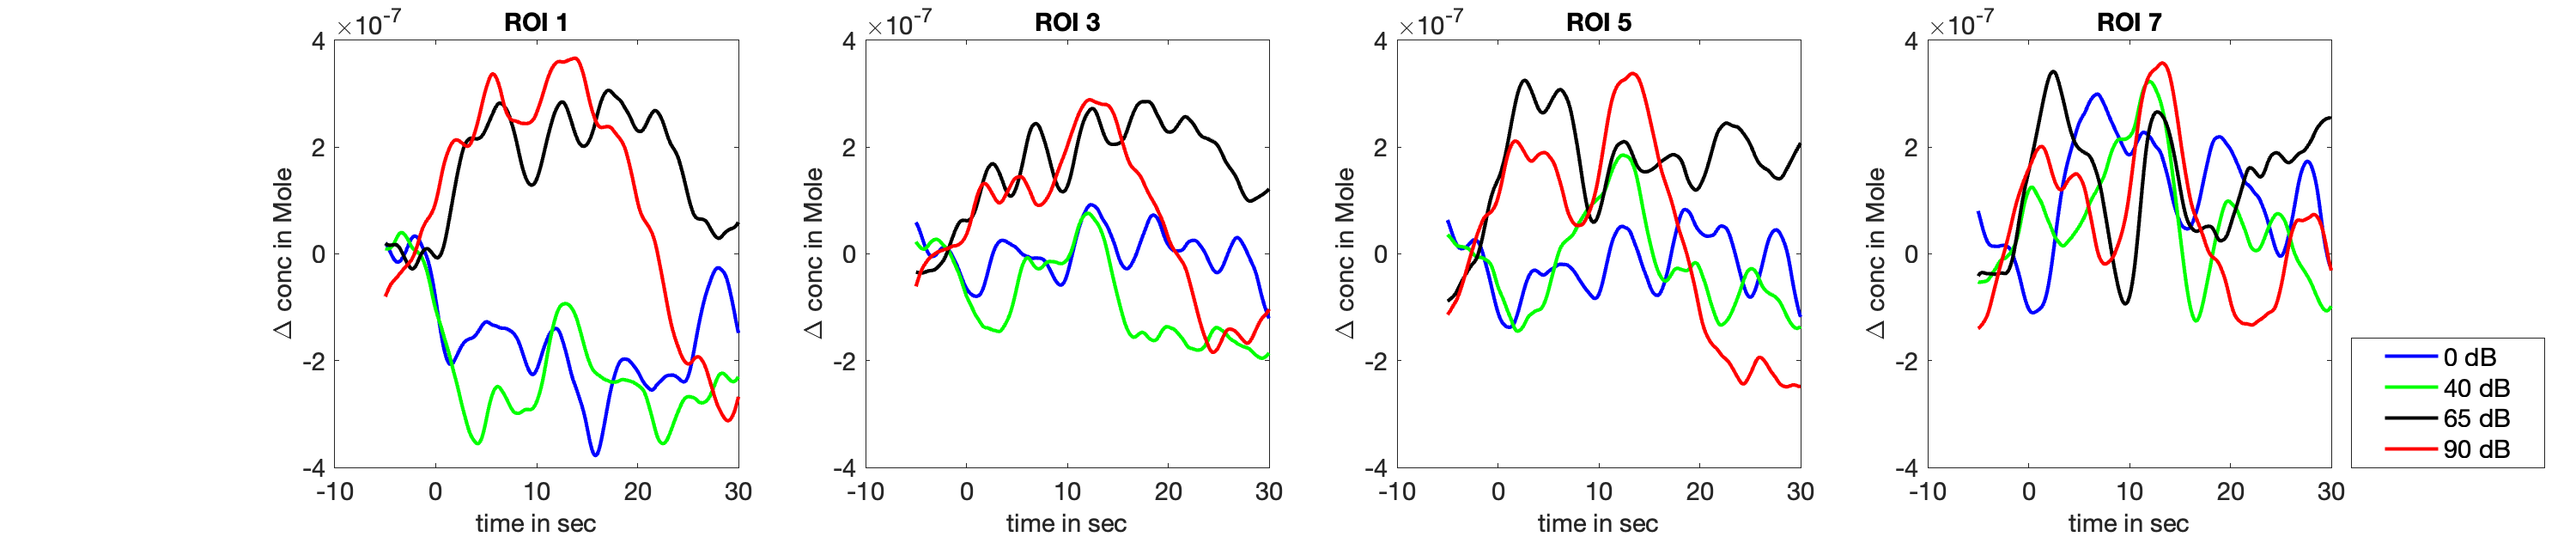
\includegraphics[scale=.29]{bilder/ROI/sub_chang_s_HbO.png}
  \caption{Measurement from participant  1.}
\end{figure}

\begin{figure}[H]
  \centering
    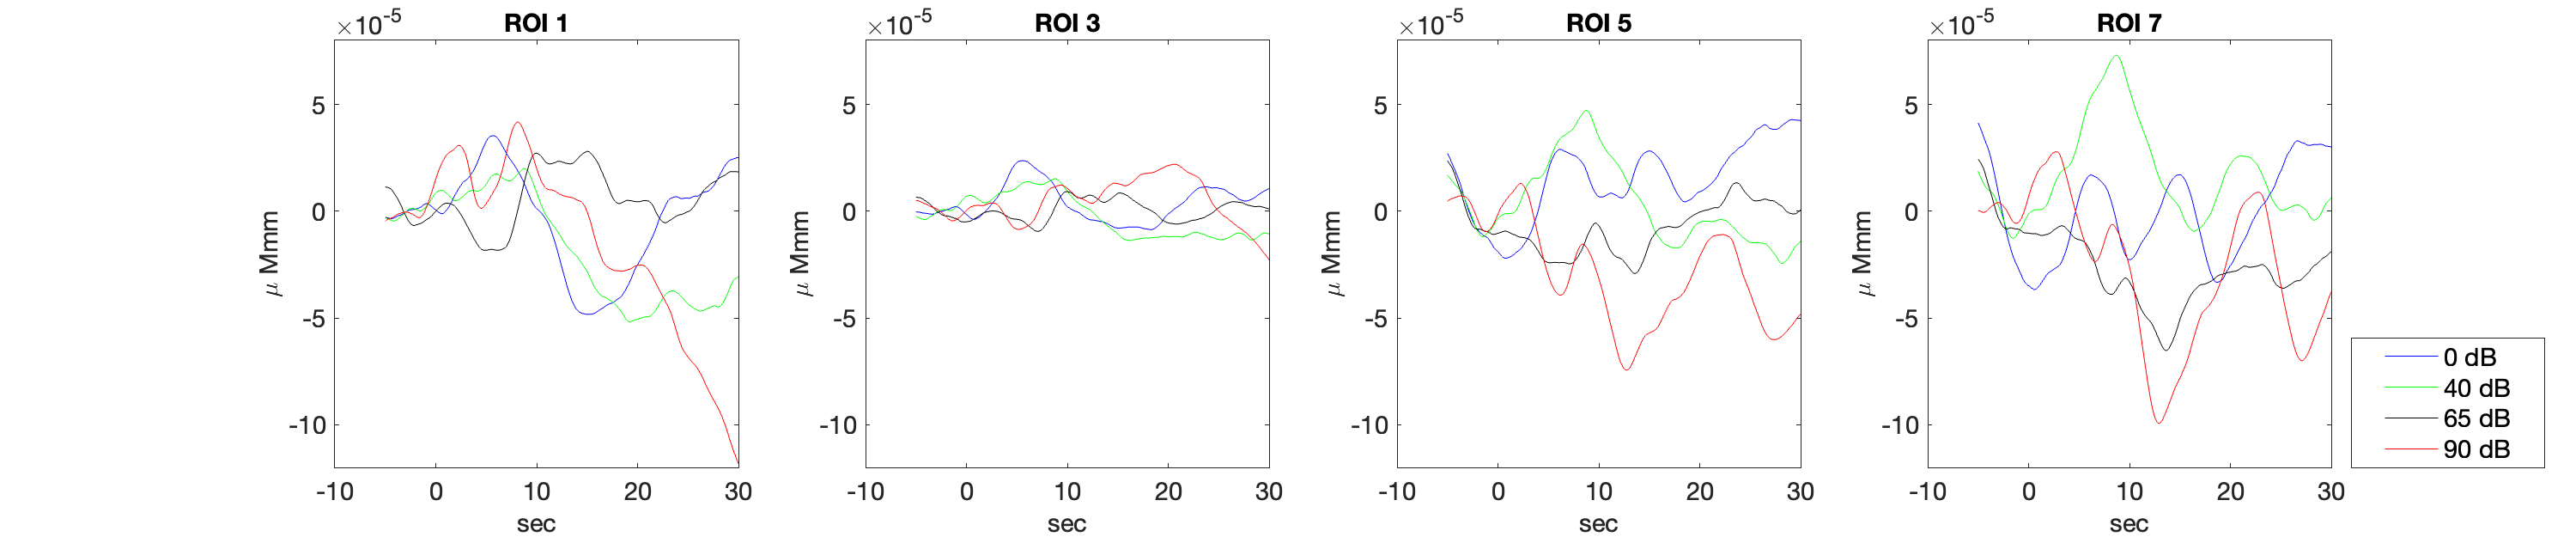
\includegraphics[scale=.29]{bilder/ROI/sub_gleb2_s_HbO.png}
  \caption{Measurement from participant  2.}
\end{figure}

\begin{figure}[H]
  \centering
    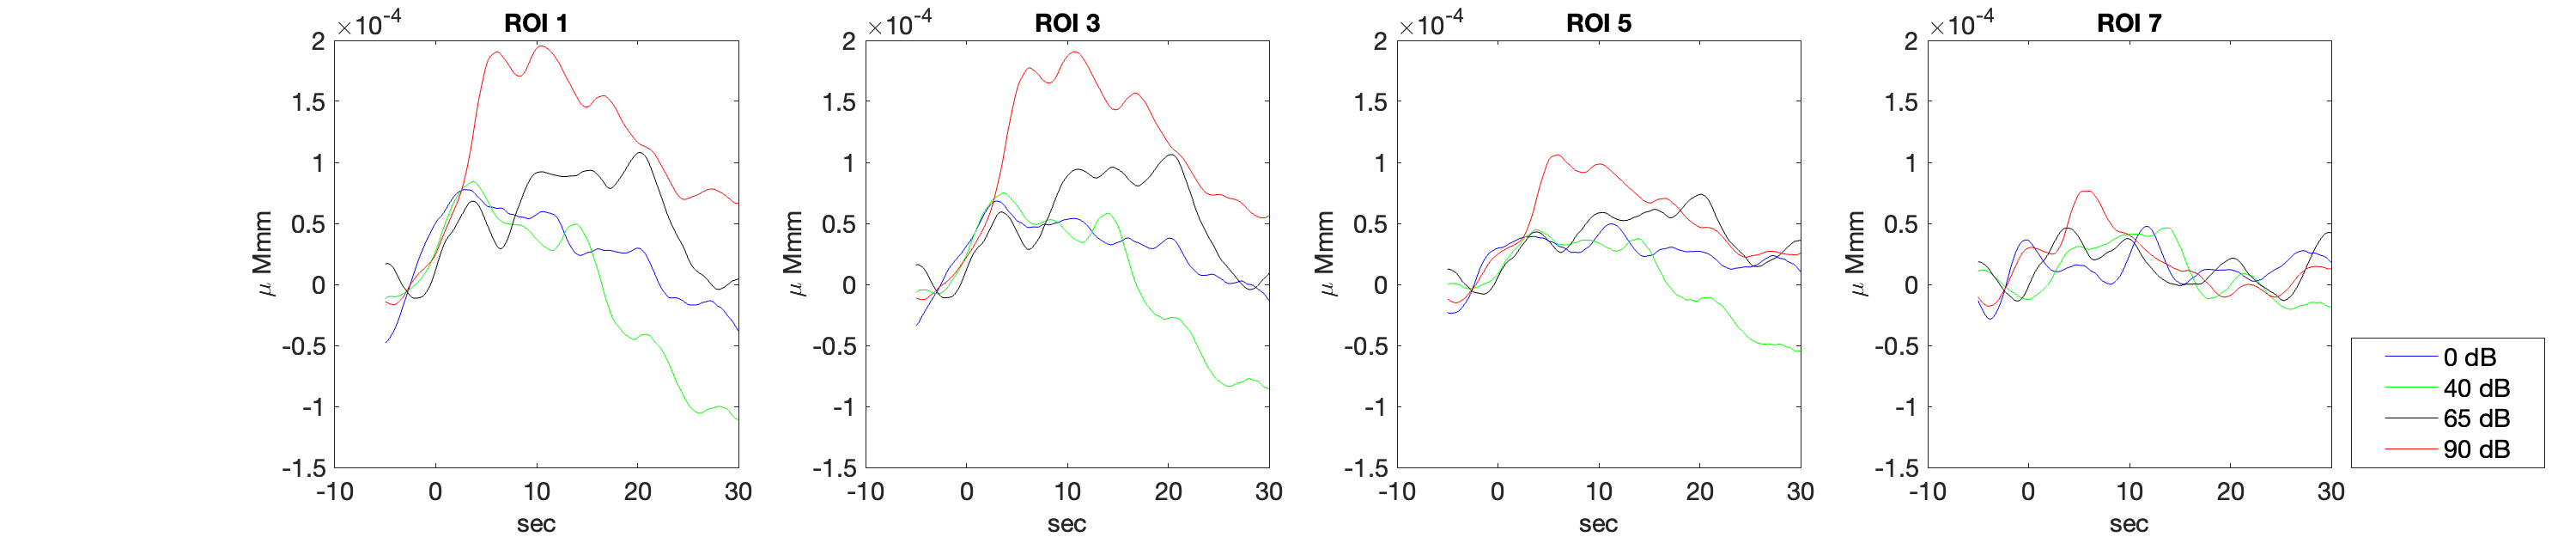
\includegraphics[scale=.29]{bilder/ROI/sub_jonas_s_HbO.png}
  \caption{Measurement from participant  3.}
\end{figure}

\begin{figure}[H]
  \centering
    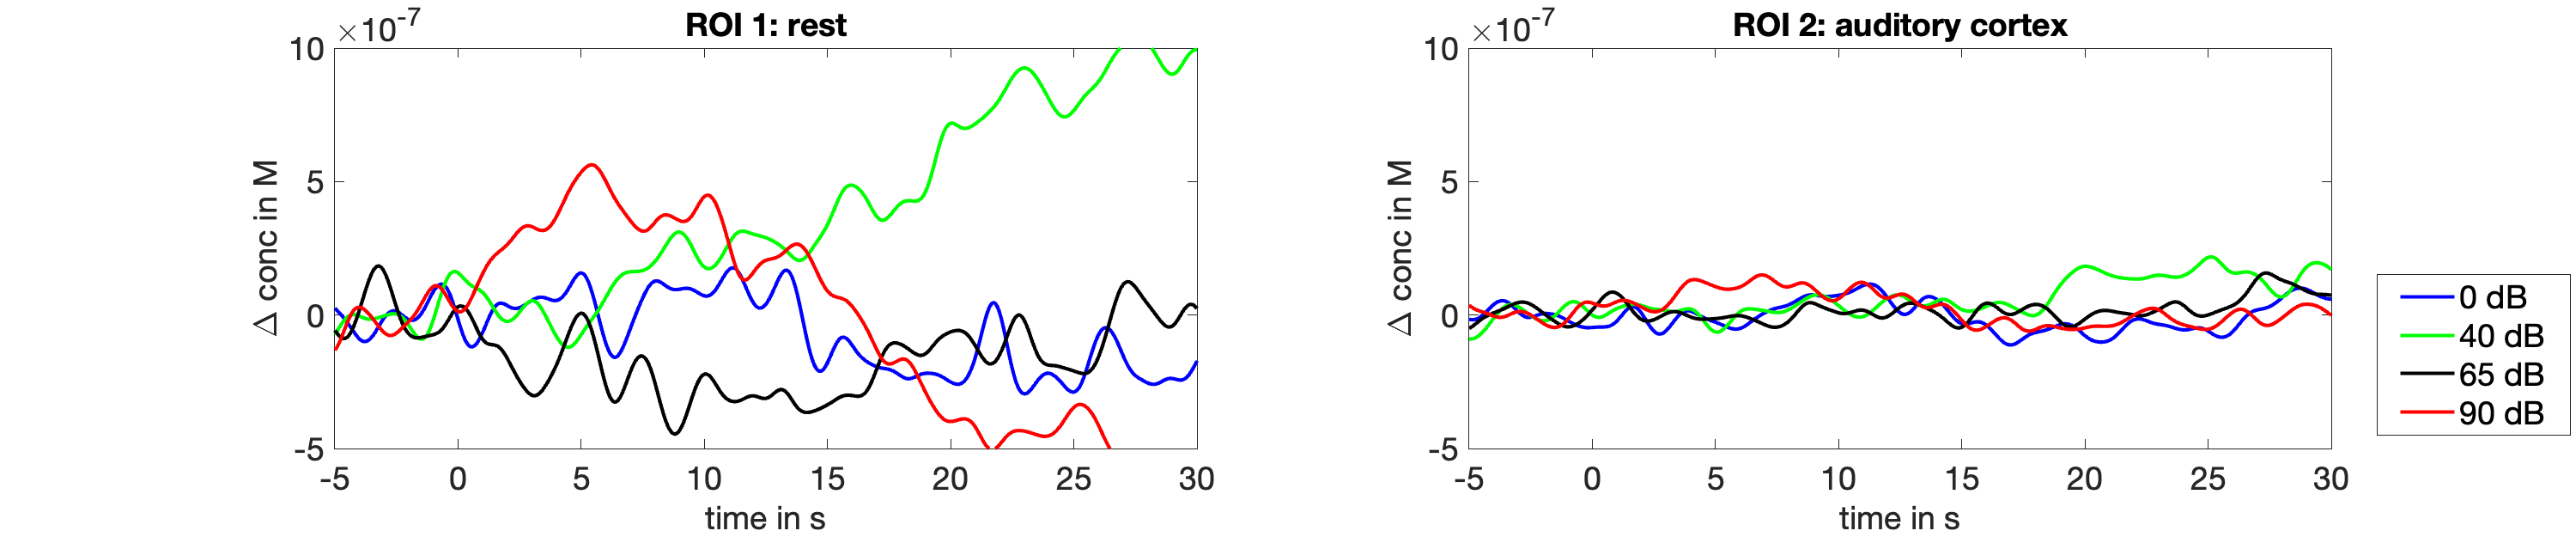
\includegraphics[scale=.29]{bilder/ROI/sub_lin_s_HbO.png}
  \caption{Measurement from participant  4.}
\end{figure}

\begin{figure}[H]
  \centering
    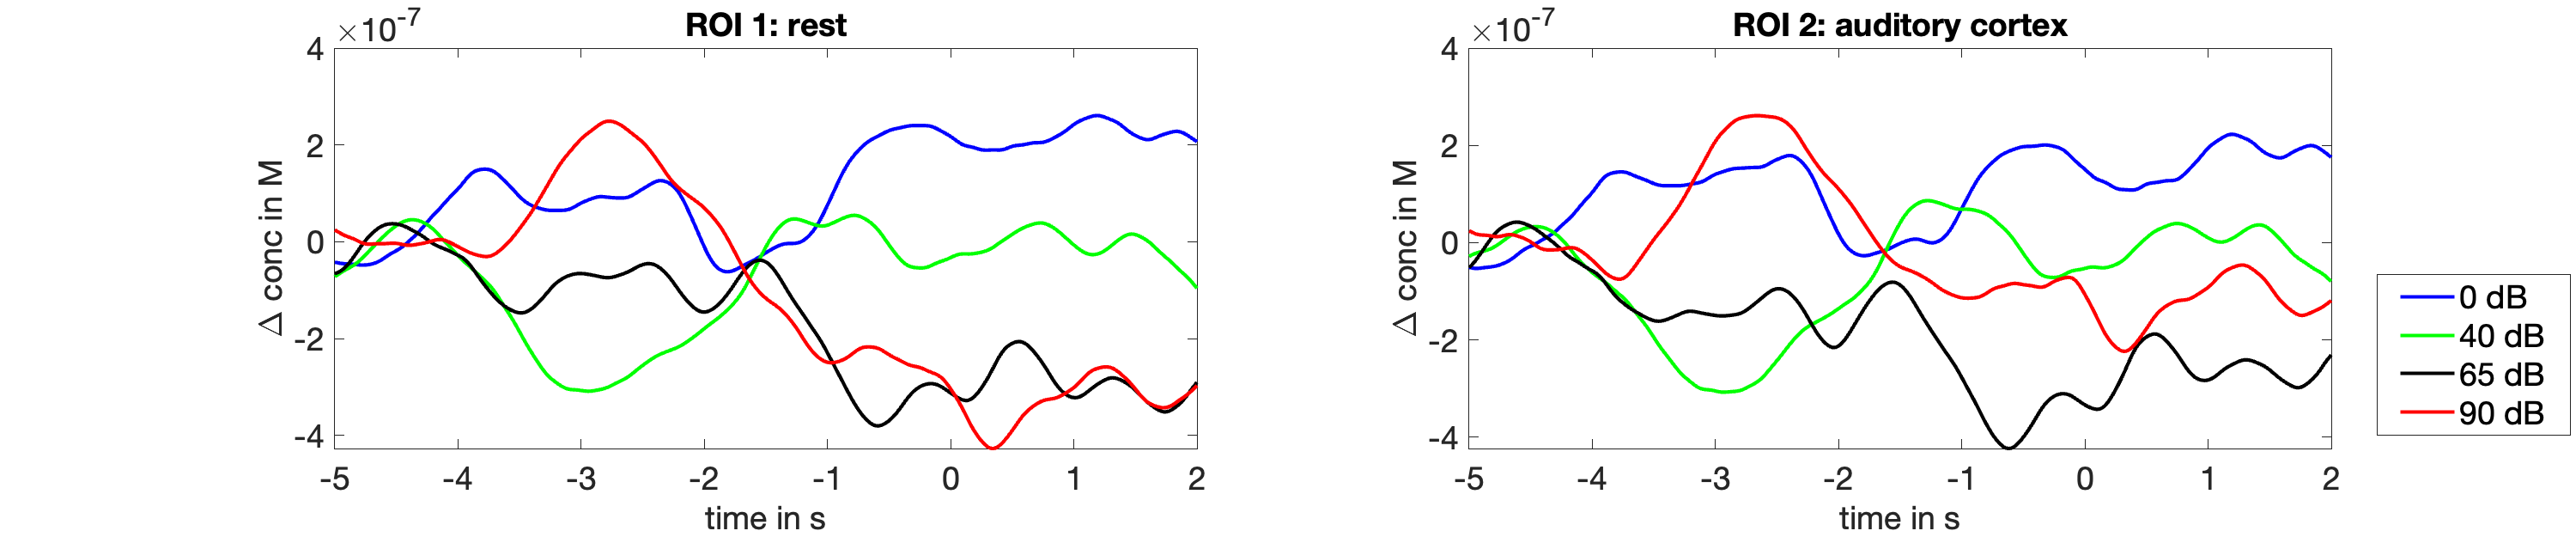
\includegraphics[scale=.29]{bilder/ROI/sub_lukas_s_HbO.png}
  \caption{Measurement from participant 5.}
\end{figure}

\begin{figure}[H]
  \centering
    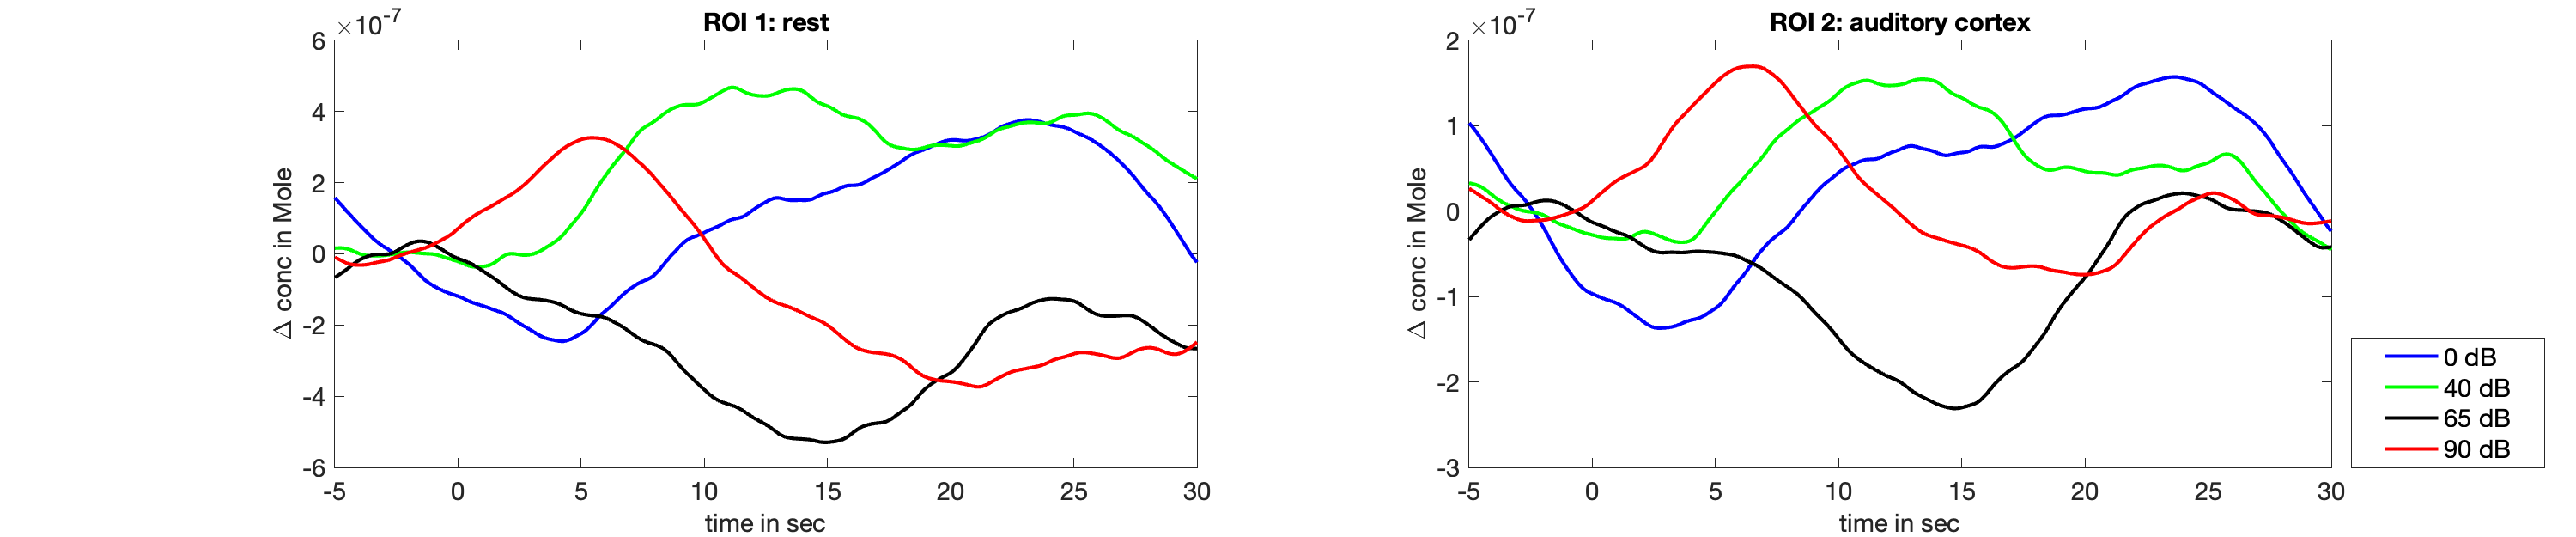
\includegraphics[scale=.29]{bilder/ROI/sub_shelia_s_HbO.png}
  \caption{Measurement from participant  6.}
\end{figure}


\begin{figure}[H]
  \centering
    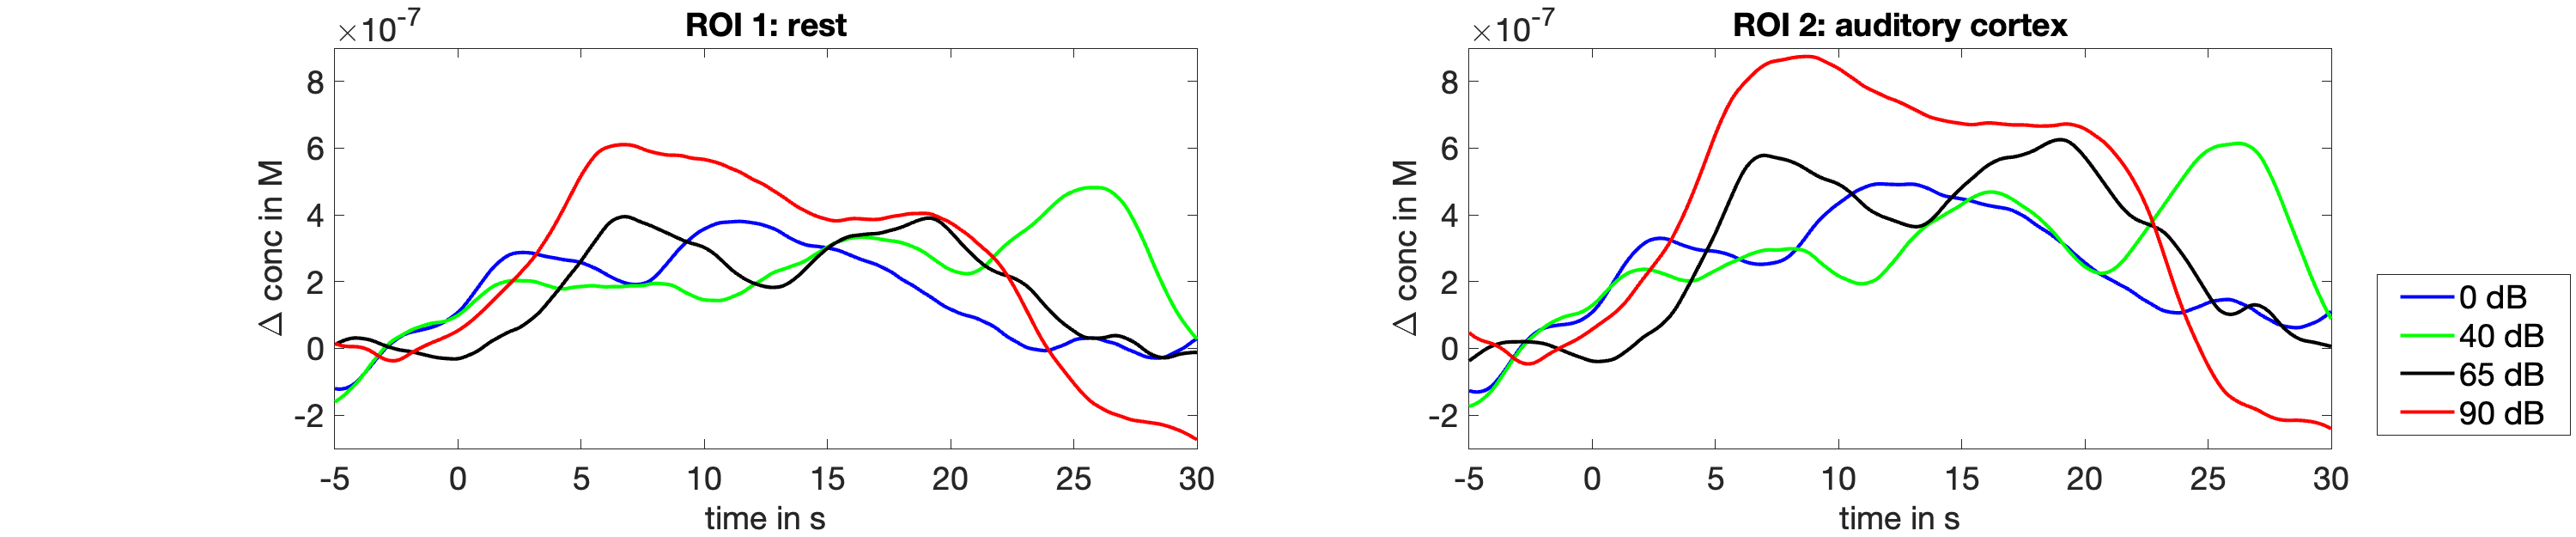
\includegraphics[scale=.29]{bilder/ROI/sub_liao_s_HbO.png}
  \caption{Measurement from participant 7.}
\end{figure}



\begin{figure}[H]
  \centering
    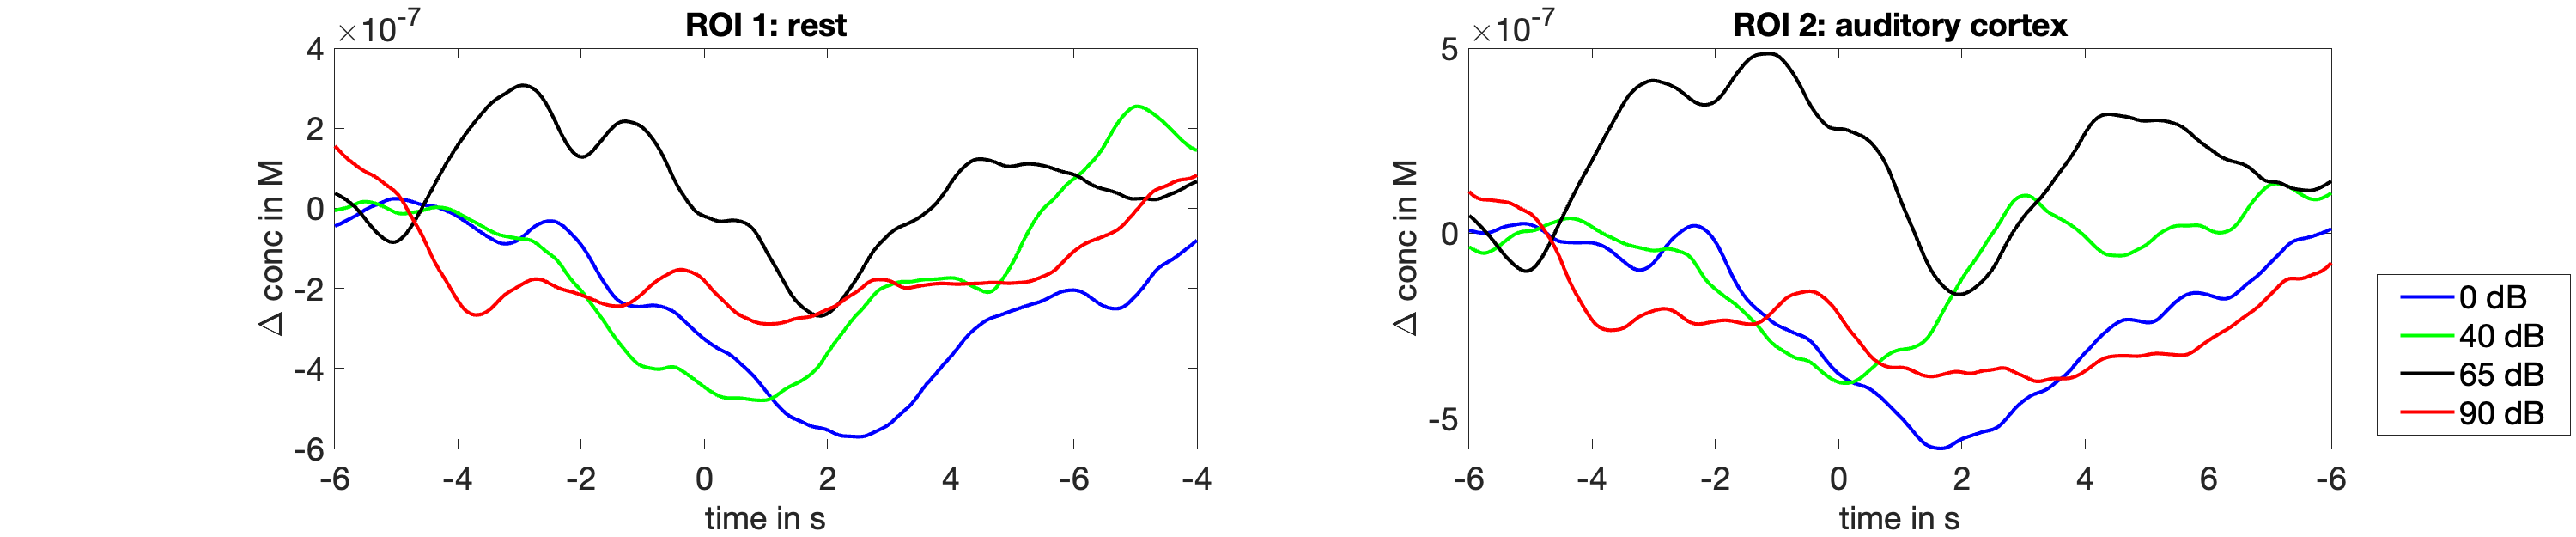
\includegraphics[scale=.29]{bilder/ROI/sub_luca2_s_HbO.png}
  \caption{Measurement from participant 8. Silent comparision.}
\end{figure}

\newpage

\section {Poor Measurements}
There were also some poor measurements even though the SCI is above the threshold 0.75. For example, in our case of participant 4. One possible reason can be due to the thick dark hair of the participant. Light absorption can affect the result greatly.

\begin{figure}[H]
  \centering
    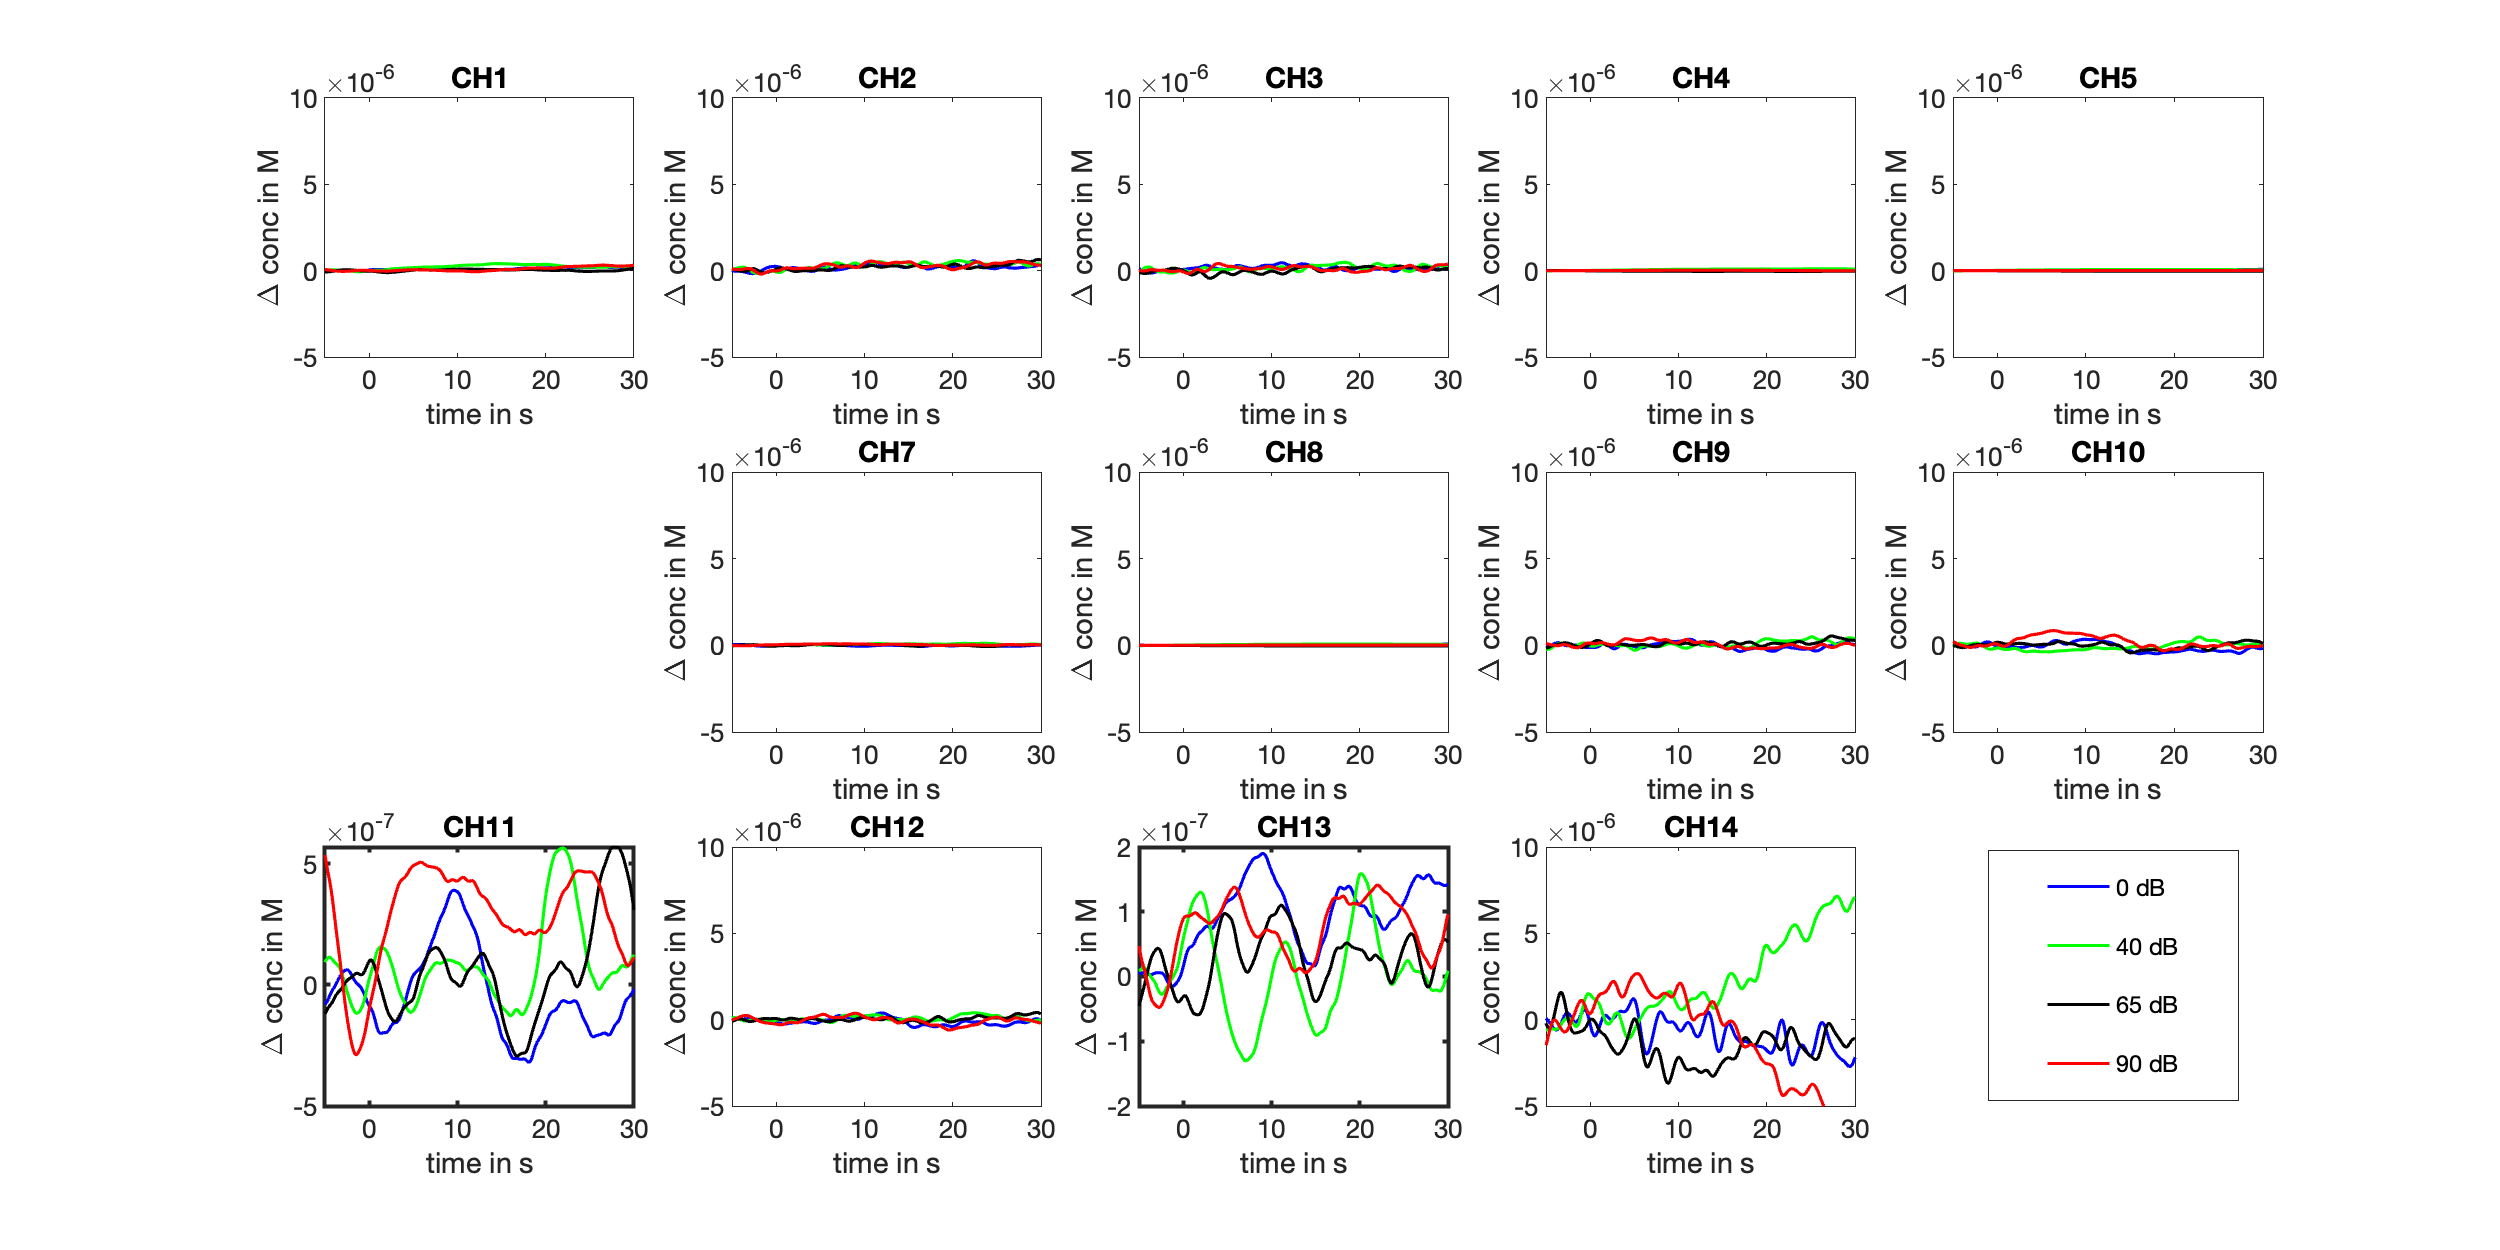
\includegraphics[scale=.35]{bilder/HbO_Mole/sub_lin_s_HbO.png}
  \caption{HbO Measurement from participant 4.}
\end{figure}


\begin{figure}[H]
  \centering
    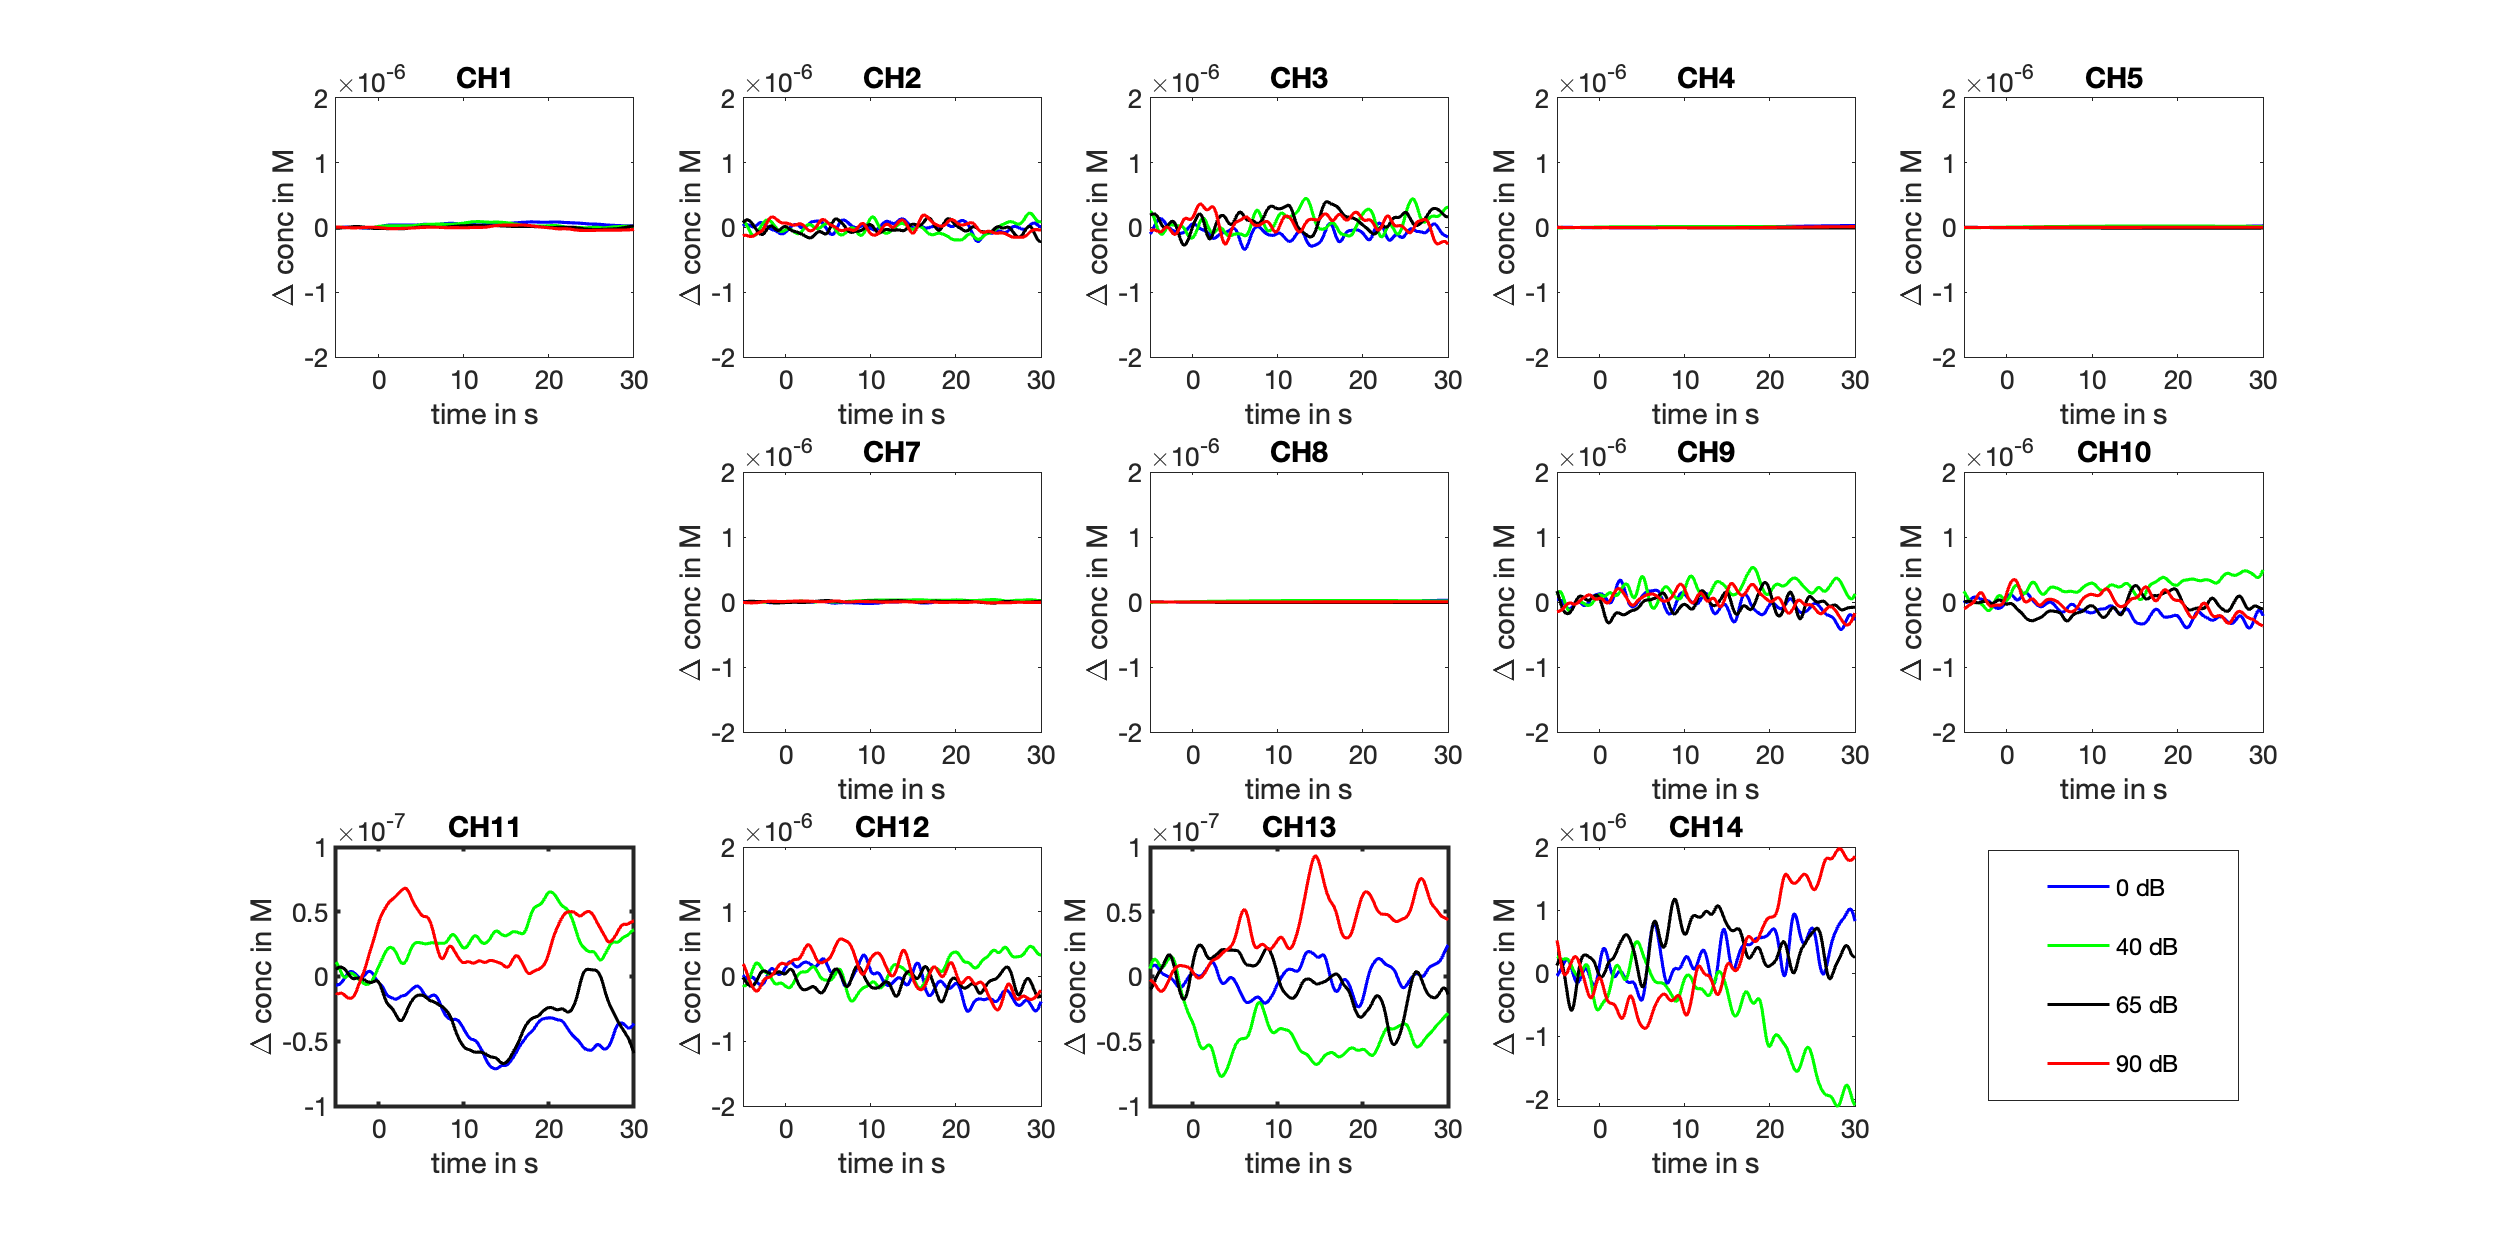
\includegraphics[scale=.35]{bilder/HbR_Mole/sub_lin_s_HbR.png}
  \caption{HbR Measurement from participant 4.}
\end{figure}

